\documentclass{../../text-style}

\texttitle{Лекция 15: Основы сетевой безопасности}

\begin{document}

\maketitle
\thispagestyle{empty}

\section{Введение}

Вообще, тема сетевой безопасности заслуживает отдельного курса, но кое-какие вещи, типа тех же сертификатов, необходимы любому программисту в повседневной работе, так что обойти их обсуждение хотя бы кратко не получится. В современном мире почти все сервисы требуют аутентификации, авторизации и обеспечения безопасности. Причём, обратите внимание, что аутентификацию и авторизацию часто путают, это разные вещи:

\begin{itemize}
    \item \textit{аутентификация} --- это установление личности (точнее, идентичности) участника взаимодействия; личность нам не важна, нам важно знать, что это тот пользователь, о котором мы думаем, или хотя бы пользователь из той группы пользователей с одинаковыми правами, за которого себя выдаёт; аутентификация часто взаимна --- сервер не доверяет клиенту, но и клиент не может быть уверен в том, что сервер не подделан злоумышленником;
    \item \textit{авторизация} --- это установление прав на выполнение операции, когда аутентификация уже выполнена. Вы можете быть вполне легитимным пользователем GMail, но это не значит, что вы имеете право просматривать мою почту; или вы можете иметь доступ только на чтение к какому-то документу.
\end{itemize}

\textit{Шифрование} --- это обеспечение конфиденциальности передаваемой информации. Но для информационной безопасности важна не только конфиденциальность, но и:

\begin{itemize}
    \item \textit{целостность} --- что злоумышленник ничего не поменял в сообщении; даже не имея возможности его прочитать, он может нанести ущерб, внеся изменения, если они не будут замечены получателем;
    \item \textit{актуальность} --- что злоумышленник не проиграл просто старое сообщение; ведь не надо ни дешифровать, ни изменять как-то ваше сообщение об оплате мобильной связи, чтобы лишить вас всех денег, если протокол оплаты не обеспечивает свойство актуальности.
\end{itemize}

При этом важно понимать, что мы уже давно не в Древнем Риме, и пытаться взломать шифр <<в лоб>> --- довольно безнадёжное занятие. Тем не менее, системы часто взламывают и сейчас --- прежде всего, используя социальные методы атаки, начиная от флешки, подкинутой работнику организации (ему же будет интересно, что там, и он обязательно воткнёт её в рабочий компьютер). Заканчивая психологическим давлением по цепочке из нескольких человек. Причём, часто эта цепочка может состоять только из одного сотрудника --- большинство попыток взлома происходит изнутри, от обиженных или даже уволенных (но по какой-то причине не удалённых из информационных систем) сотрудников. В общем, защищаться надо от атак не только и не столько извне.

Кроме того, в отличие от обычной разработки программного обеспечения, сетевая безопасность --- это игра против живого, умного и часто хорошо оснащённого противника, которому, к тому же, принадлежит инициатива, настолько, что вы часто не сможете даже понять, что вас атаковали. Поэтому задача обеспечения безопасности никогда не формулируется как <<сделать взлом невозможным>> --- скорее это задача сделать стоимость взлома большей, чем выгода, приобретаемая взломщиком. Из этого, кстати, следует, что если ваша система никаких ценных данных не содержит, то и защищать её особо не стоит. И это на самом деле довольно важное соображение, поскольку безопасность неизбежно вступает в конфликт с удобством использования. Простой пример неверного решения: Blackboard, там после пары часов неактивности токен авторизации протухает и надо логиниться снова. Хотя, казалось бы, Blackboard --- не банковское приложение, и мог бы доверять компьютеру пользователя больше (скажем, как вконтакт, доверял бы токену хотя бы пару месяцев). Внезапные требования залогиниться крайне раздражают.

И главное правило сетевой безопасности --- не придумывать свои шифры и протоколы. За протоколами безопасности стоит большая наука, и самодельный на коленке протокол, сколь бы хитрым он вам ни казался, может иметь очевидные для специалистов уязвимости и быть взломан за пару часов. Придумывать свой хитрый шифр или протокол аутентификации --- в общем случае очень плохая идея.

Большая часть дальнейшего рассказа будет по соответствующей главе в замечательной книге Э. Таненбаума, Д. Уэзеролл <<Компьютерные сети>> (очень рекомендую).

\section{Шифрование}

Классическая схема шифрования предполагает передачу конфиденциальных данных по каналу, который может прослушивать злоумышленник (так называемая схема с пассивным злоумышленником) или злоумышленник может модифицировать сообщения в канале (схема с активным злоумышленником):

\begin{center}
    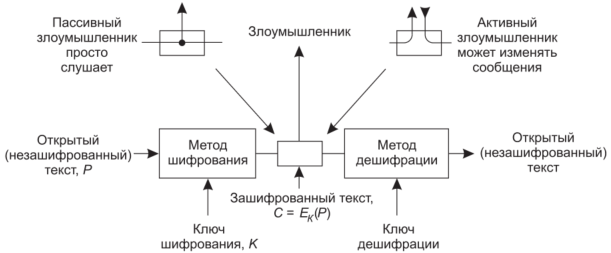
\includegraphics[width=0.8\textwidth]{cryptography.png}
    \attribution{Э. Таненбаум}
\end{center}

Незашифрованный текст называется в англоязычной литературе Plaintext и поэтому обозначается P. Зашифрованный текст называется Ciphertext и обозначается C. Алгоритм шифрования (Encryption, E) использует параметр K (Key) --- ключ шифрования, по которому преобразует открытый текст в зашифрованный: $C = E_K(P)$. Алгоритм дешифрования (Decryption, D) использует ключ дешифрации (тот же, или отличающийся от K), чтобы построить обратно открытый текст по его зашифрованному варианту.

\noindent\begin{minipage}{\textwidth}
    \begin{minipage}[c][4cm][c]{\dimexpr0.7\textwidth-0.7\Colsep\relax}
        В криптографии традиционно считается, что сам алгоритм шифрования известен, неизвестен только ключ. Связано это с тем, что хороший алгоритм шифрования разработать сложно (это занимает годы) и если его взломают, придётся менять и сам алгоритм, и его программные и аппаратные реализации. Это сложно и дорого. Если взломают ключ, достаточно выбрать другой. Более того, современные алгоритмы заранее меняют ключи раз в несколько секунд, чтобы осложнить злоумышленнику криптоанализ.
    \end{minipage}\hfill
    \begin{minipage}[c][4cm][c]{\dimexpr0.3\textwidth-0.3\Colsep\relax}
        
\includegraphics[width=0.7\textwidth]{youAreBeingWatched.png}
    \end{minipage}%
\end{minipage}

Ещё стоит помнить, что алгоритмы шифрования --- это суровая алгебра, теория чисел и теория вероятностей. Если вы думаете, что криптосхема <<кручу-верчу, запутать хочу>> или последовательное применение двадцати разных алгоритмов шифрования повысит криптостойкость вашего метода шифрации, вас могут ждать неприятные сюрпризы (вплоть до того, что криптостойкость внезапно понизится). Повысить криптостойкость можно увеличением размера ключа, но во многих странах существуют законодательные ограничения на длину ключа в гражданских шифрах. Связано это не с тем, что тоталитарный режим хочет следить за всеми своими гражданами (хотя хочет, конечно), а с тем, что при крайней необходимости (например, постановлении суда) и затратой больших вычислительных ресурсов (например, суперкомпьютера ВМК МГУ) сообщение всё-таки можно было бы расшифровать. Военные шифры имеют такую длину ключа, что дешифровка сообщений по крайней мере грубой силой на всех нынешних и будущих вычислительных ресурсах планеты даже по оптимистичным оценкам займёт время большее, чем нужно Солнцу, чтобы исчерпать запасы водорода и погаснуть.

\subsection{Шифрование с симметричным ключом}

Подавляющее большинство интернет-трафика шифруется шифрами с симметричным ключом (то есть ключом, одинаковым для шифровки и дешифровки), потому что они работают очень быстро. Обратите внимание, речь идёт не о шифровании секретных донесений шпионов или банковских переводов, а о шифровании вообще всего трафика --- любой веб-страницы, скачиваемых файлов и даже фильмов, которые вы смотрите через стриминговые сервисы (казалось бы, что секретного в фильме, который и так может посмотреть любой желающий, но если посторонние узнают тот факт, что вы его смотрите --- это privacy violation). А это десятки гигабайт трафика, шифруемых/дешифруемых в реальном времени. Поэтому современные процессоры имеют даже аппаратную поддержку симметричных шифров. 

Обычно прикладные программисты симметричные шифры используют просто как чёрный ящик, куда можно скормить данные и ключ, и получить зашифрованные/расшифрованные данные. Реализовывать алгоритмы шифрования \emph{не нужно}, есть хорошие библиотеки (OpenSSL для C, а следовательно и для любых языков, которые могут вызывать сишный код, для .NET и Java более высокоуровневая библиотека с забавным названием Bouncy Castle для криптографических изысков, а распространённые шифры .NET поддерживает и в стандартной библиотеке --- см. пространство имён System.Security.Cryptography). Однако общее понимание того, как работают симметричные шифры, что такое режимы шифрования, IV и прочие страшные вещи, знать всё равно надо, иначе даже чтение документации вызовет сильную боль.

Один из первых массово используемых в сети гражданских симметричных шифров --- Data Encryption Standard, появившийся аж в 1975 году (задолго до собственно сети) по заказу правительства США (естественно). Он использовал 56-битный ключ, что для 1975 года было ок, однако в 1999 году такие шифры ломались за часы, и Таненбаум писал, что в конечном итоге на базаре можно было купить устройство, ломавшее DES чуть ли не на лету. Поэтому... в 1995 году кому-то пришла в голову идея утроить длину ключа от DES, просто применив DES трижды, так появился Triple DES. При этом применялась схема шифрования $ciphertext = E_{K3}(D_{K2}(E_{K1}(plaintext)))$, что позволяет выбрать $K1 = K2$ и работать со старыми устройствами, которые умеют только одинарный DES. Triple DES и по сей день является вполне достойной опцией для гражданского шифрования, однако поскольку он был разработан Большими Корпорациями По Заказу Правительства, параноидальное по природе криптографическое сообщество его не любит. На смену ему в 2001 году пришёл Advanced Encryption Standard (AES, также известный под своим оригинальным названием, Rijndael), который хоть и утверждён как стандарт всё тем же правительством США, разработан двумя бельгийскими криптографами в рамках открытого конкурса, и принято считать, что этот шифр не может содержать в себе backdoor-ов специально для Дядюшки Сэма. Поскольку он сам по себе неплох и довольно криптостоек (использует ключи длины 128, 192 или 256 бит), он получил широкое распространение и сейчас пользуются в основном им.

Все симметричные шифры концептуально устроены одинаково. Вот, например, DES (как самый простой):

\begin{center}
    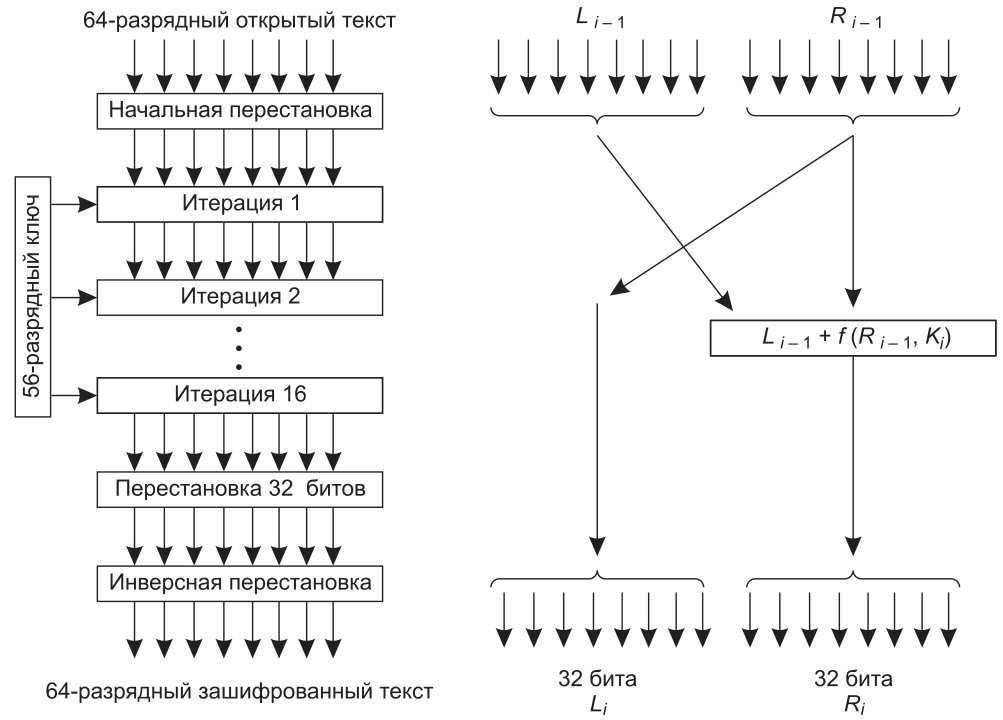
\includegraphics[width=0.6\textwidth]{des.png}
    \attribution{Э. Таненбаум}
\end{center}

Задача шифра --- как можно лучше перемешать биты входного сообщения, как можно сильнее <<примешав>> к ним биты ключа, чтобы каждый бит выходного сообщения зависел (ао возможности) от каждого бита входного сообщения и каждого бита ключа. Для этого выполняется перестановка (по известной схеме, не зависящая от ключа, её цель --- перемешать биты, не более), дальше выполняется 16 итераций по следующей схеме: берётся 64-битный блок текста (если длина текста на 64 не делится, он дополняется нулями), последние 32 бита становятся первыми 32 битами результата без каких-либо преобразований, первые 32 бита хитро xor-ятся с битами ключа и правой частью блока. Результат всех 16 таких перестановок снова перемешивается и подаётся на выход как зашифрованный текст. Подозреваю, что доказывать статистические свойства результирующей битовой последовательности --- настоящий ад, но необходимо для проверки криптостойкости шифра, именно поэтому разрабатывать свой шифр --- плохая идея.

\subsection{Режимы симметричного шифрования}

Симметричное шифрование интересно тем, что самый надёжный шифр, который вообще невозможно взломать --- одновременно и самый простой. Достаточно в качестве ключа взять случайную битовую последовательность, равную длине передаваемого текста, и побитово xor-ить их (то есть применить операцию <<исключающее или>>, которая интересна тем, что a xor b xor b = a). Однако в таком случае возникает задача передачи ключа, которая не проще, чем передача сообщения. В принципе, шпион, уезжая на задание, может взять с собой SSDшку с парой терабайт ключа, и отправлять донесения, пока он не кончится, и расшифровать их будет нельзя, потому что по статистическим свойствам передаваемый сигнал не отличим от белого шума. Но если речь идёт о шифровании всего трафика в интеренете, это не вариант. Поэтому ключи имеют ограниченные размеры (кстати, законы большинства стран запрещают использовать длинные ключи для гражданских целей, чтобы если таки возникнет необходимость что-то расшифровать, это было можно, хоть и трудно, сделать). А поэтому есть разные способы применить ограниченной длины ключ для шифрования сообщения произвольной длины.

\subsubsection{Electronic Code Book, ECB}

Первый способ, приходящий в голову --- это разбить текст на блоки и применять ключ к каждому блоку последовательно. Этим мы фактически получаем подстановочный шифр (в духе шифра Цезаря, который шифровал сообщение циклическим сдвигом букв по алфавиту), но над алфавитом из символов $2^{длина\ ключа}$. Что при достаточной длине ключа хорошо, но всё-таки при больших объёмах передаваемых данных страдает тем же, чем и шифр Цезаря --- уязвимостью к статистической атаке. Мы можем заранее посчитать вероятности встречи в незашифрованных данных тех или иных блоков, потом посчитать в зашифрованном тексте частоты, с которыми встречаются блоки, и найти ближайшее соответствие. Тем более что злоумышленнику не обязательно даже дешифровать сообщение: 

\begin{center}
    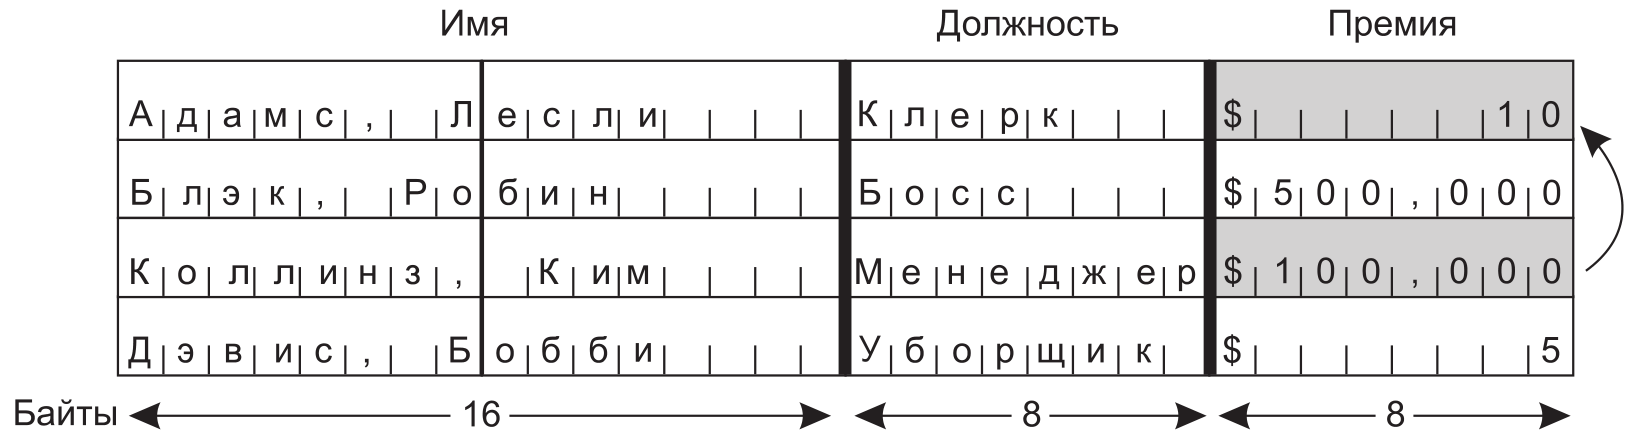
\includegraphics[width=0.85\textwidth]{ecbAttack.png}
    \attribution{Э. Таненбаум}
\end{center}

Положим, Адамс Лесли знает, что компания распределяет большую годовую премию, но поскольку он всего лишь обычный клерк, он почти ничего не получит. Однако он смог перехватить зашифрованную платёжную ведомость, которую начальник хотел отправить в банк, знает формат записи, и знает, что сотрудники там перечислены в алфавитном порядке. Ему достаточно просто поменять местами два блока (не с записью начальника, это наверняка вызовет непонимание уже в банке), чтобы стать богаче на 99990 долларов, хотя он так и не узнает, кому сколько должны были заплатить.

Поэтому ECB в реальной жизни практически не применяется.

\subsubsection{Cipher Block Chaining, CBC}

Схема, надёжно защищающая и от статистической атаки, и от атаки перестановкой --- это Cipher Block Chaining, идея которой состоит в том, что перед применением ключа следующий блок xor-ится с предыдущим зашифрованным блоком:

\begin{center}
    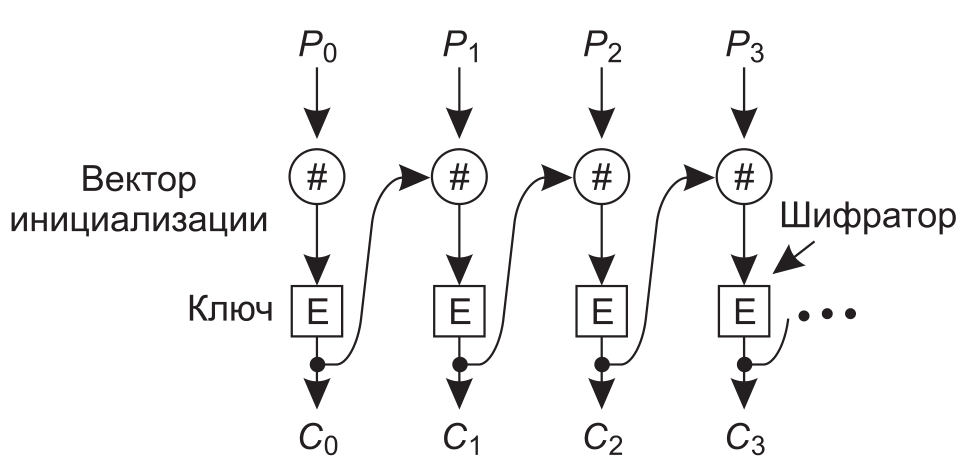
\includegraphics[width=0.6\textwidth]{cbc.png}
    \attribution{Э. Таненбаум}
\end{center}

Первый блок xor-ить не с чем, поэтому берётся просто фиксированный набор битов, называемый <<вектор инициализации>> (Initialization Vector, IV), и первый блок xor-ится с ним. IV не секретен и обычно просто жёстко вшивается в приложение.

Такая схема весьма криптостойка, однако имеет один важный на практике недостаток: если испортится хотя бы один бит зашифрованного сообщения, всё сообщение после этого бита расшифровать не получится. Правда, это же в каком-то смысле и достоинство --- принимающий точно будет знать, что кто-то пытался что-то поменять в сообщении, в отличие от ECB, где изменение может пройти незамеченным.

\subsubsection{Stream Cipher Mode, SCM}

Следующая схема не имеет проблем со случайной порчей данных --- Stream Cipher Mode, SCM. Идея в том, что мы можем сгенерировать ключ сколь угодно большой длины, просто шифруя Initialization Vector обычным коротким ключом снова и снова. После чего можно полученный ключ просто xor-ить с передаваемым сообщением: 

\begin{center}
    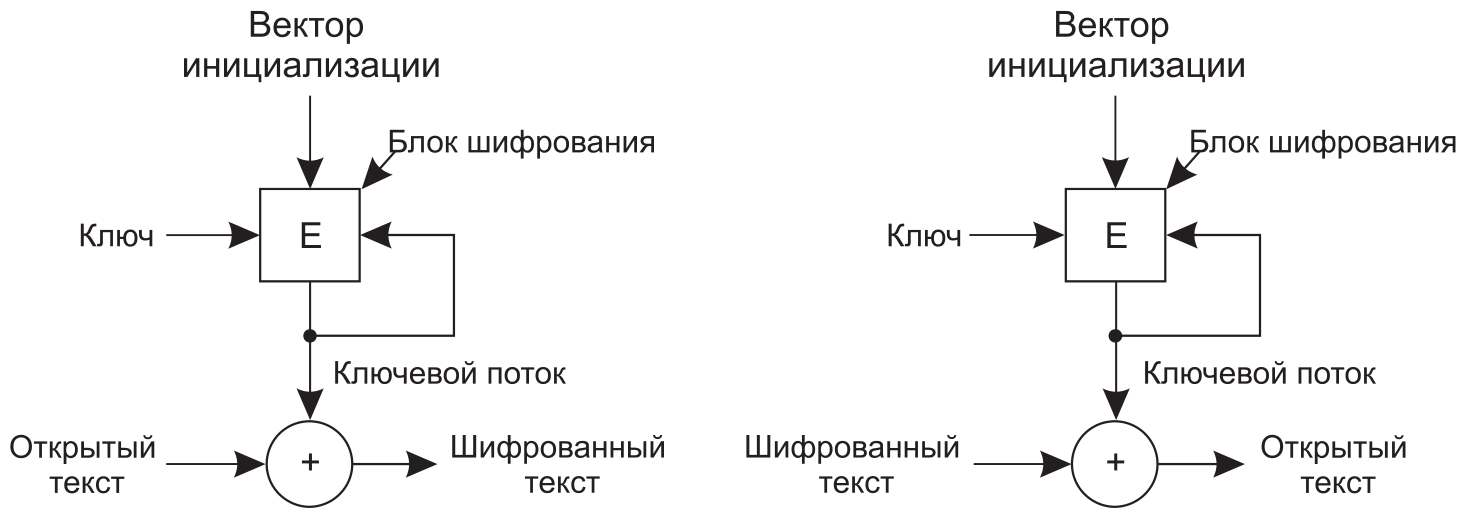
\includegraphics[width=0.85\textwidth]{scm.png}
    \attribution{Э. Таненбаум}
\end{center}

Преимущество такой схемы в том, что и отправитель, и получатель могут заранее сгенерировать себе тот самый Cipher Stream (его обычно называют keystream), и догенерировать его по мере приёма сообщения, что позитивно сказывается на скорости работы, особенно в случае передачи по сети, где сообщение появляется не сразу. Генерация ключа вычислительно сложна, но не зависит в этом случае от сообщения, а xor вычислительно очень прост (буквально одна инструкция), так что задача легко параллелится.

К тому же, порча одного бита при передаче приведёт только к порче одного бита дешифрованного сообщения. Однако криптостойкость такой схемы несколько хуже --- во-первых, keystream всё-таки определяется целиком начальным ключом (хоть он и довольно случаен, число возможных keystream-ов ограничено и они не совсем случайны, что, наверное, могут использовать умные криптоаналитики). И никогда-никогда нельзя использовать один и тот же keystream для передачи (то есть по сути, ключи надо менять каждый раз), потому что SCM уязвим к Keystream Reuse Attack: $(P_0 \oplus K_0) \oplus (Q_0 \oplus K_0) = P_0 \oplus Q_0$, где $P_0$ и $Q_0$ --- незашифрованные тексты, $K_0$ --- поток ключей.  $P_0 \oplus Q_0$, не зная $P_0$ и $Q_0$, прочитать тоже сложновато, но тут уже применима обычная статистическая атака, поскольку $P_0$ и $Q_0$ --- это обычные тексты, имеющие типичные статистические распределения.

\subsubsection{Counter Mode, CM}

Следующий режим шифрования ещё менее криптостоек, чем предыдущий, но удобен, если нам надо обеспечить произвольный доступ к частям сообщения без полной расшифровки. Типичный пример --- зашифрованные файловые системы, где надо уметь считать расшифрованный блок с диска, не расшифровывая при этом два терабайта данных, что перед ним (и не генерируя ключевой поток такой длины). Для этого используется несколько упрощённый аналог схемы SCM:

\begin{center}
    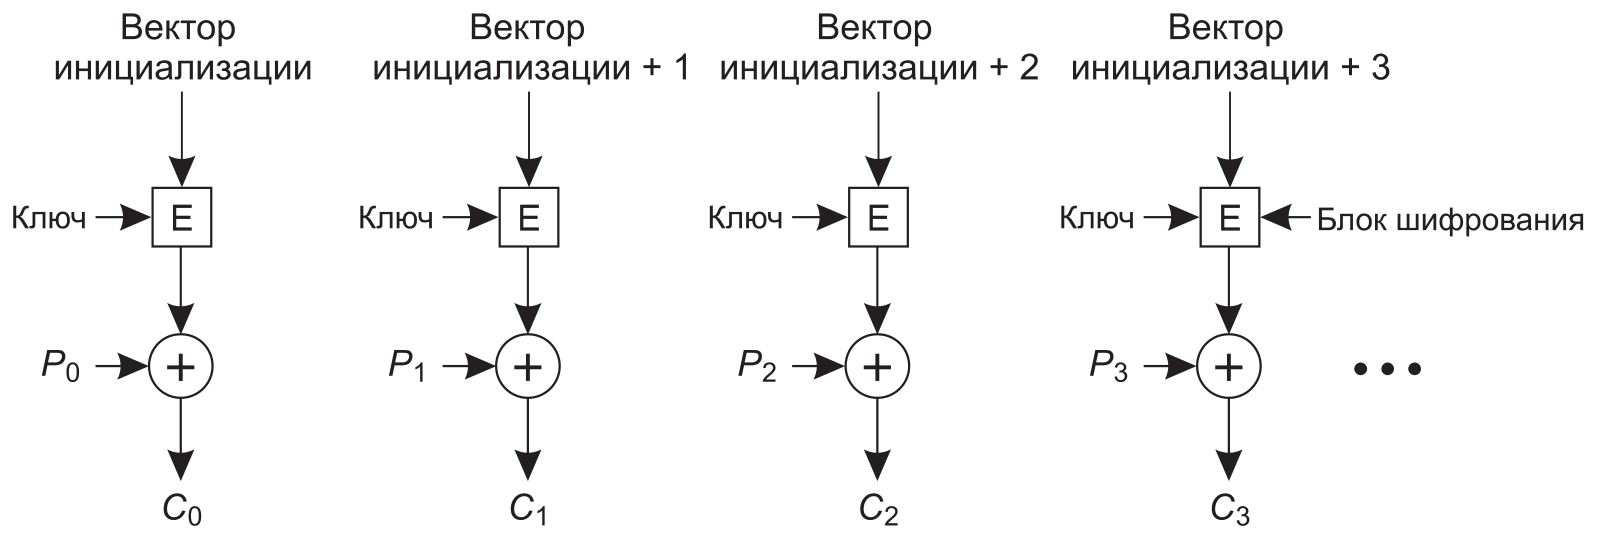
\includegraphics[width=0.85\textwidth]{cm.png}
    \attribution{Э. Таненбаум}
\end{center}

Тут мы шифруем ключом вектор инициализации, вектор инициализации + 1, вектор инициализации + 2 и т.д., рассматривая вектор инициализации просто как длинное двоичное число (и не боясь арифметического переполнения, поскольку операции в кольце по модулю $2^{длина\ IV}$ нас вполне устраивают). А дальше, как обычно, xor-им получившиися блок с открытым текстом. Расшифровать произвольный блок в таком случае можно за константное время, при этом мы всё ещё защищены от статистической атаки, поскольку каждый блок шифруется своим ключом (хоть они, как и раньше, все выводятся из начального ключа, и тут даже по очень простому алгоритму). Напомним, что IV --- не секрет.

\subsection{Алгоритм Диффи-Хеллмана}

Когда говорят о секретном ключе, обычно имеется в виду, что участники взаимодействия заранее договорились о секретном ключе и как-то выбрали его по защищённому каналу связи (например, встретились в тёмном переулке и обменялись флешками с ключами). Но магия теории чисел позволяет договориться об общем секретном ключе по открытому каналу, прямо на глазах у злоумышленника, с помощью алгоритма Диффи-Хеллмана:

\begin{center}
    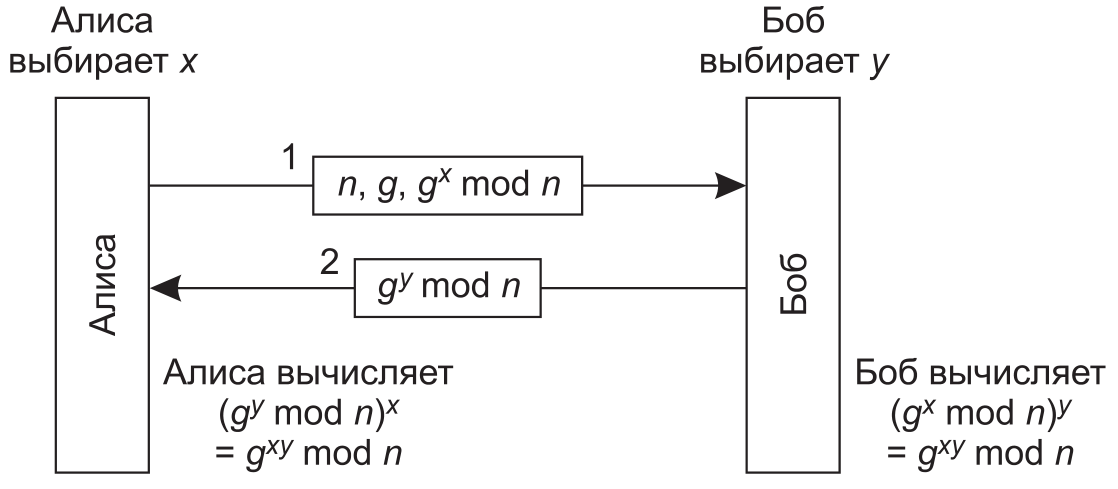
\includegraphics[width=0.6\textwidth]{diffieHellman.png}
    \attribution{Э. Таненбаум}
\end{center}

Алиса и Боб загадывают по случайному числу\footnote{Загадывают не сами Алиса и Боб, конечно, а генератор случайных чисел того софта, который они используют, чтобы общаться.}, а также выбирают достаточно большие числа n и g (они могут даже не выбирать их сами, они могут быть захардкожены в коммуникационной программе). Алиса отправляет Бобу $n$, $g$ и $g^x\ mod\ n$. Боб отвечает Алисе $g^y\ mod\ n$. Секретный ключ --- это $g^{xy}\ mod\ n$. Как нетрудно убедиться, и Алиса, и Боб без труда могут его вычислить. Однако злоумышленник, даже перехватив оба сообщения и зная n, g, $g^x\ mod\ n$ и $g^y\ mod\ n$ не может посчитать ни $g^{xy}\ mod\ n$, ни $x$, ни $y$, по крайней мере за разумное время. Для этого ему пришлось бы решать задачу дискретного логарифмирования в кольце вычетов по модулю $n$, а сейчас считается, что эта задача полиномиального решения не имеет, и на ней базируется также протокол шифрования с открытым ключом ElGamal (так что если злоумышленник --- гений алгебры, он получит не только ваш секретный ключ, но и уничтожит большой пласт современной криптографии, заодно получив ряд престижных наград).

Диффи-Хеллман используется, например, в Телеграм для установления зашифрованного соединения в приватных чатах, так что даже если провайдер пользователей продался Роскомнадзору и дешифрует HTTPS-трафик, прочитать сообщения он не сможет. Публичные чаты (которыми пользуется подавляющее большинство пользователей Телеграм) ничего такого не делают и полагаются на HTTPS. Кстати, HTTPS тоже иногда использует Диффи-Хеллмана для установления соединения и определения симметричного ключа для шифрования трафика.

Плохая новость в том, что алгоритм Диффи-Хеллмана работает, только если уже выполнена взаимная аутентификация, то есть Алиса уверена, что говорит с Бобом, а Боб --- с Алисой. Иначе секретный ключ за них обоих может выбрать злоумышленник с помощью атаки посредника (<<Man in the middle>>):

\begin{center}
    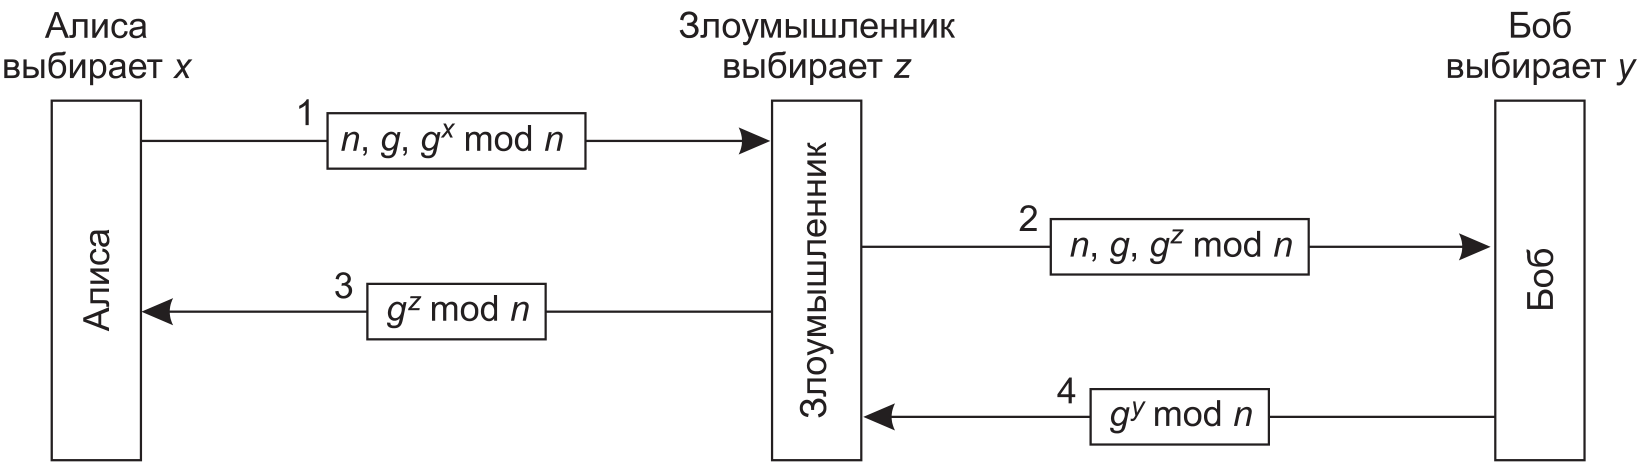
\includegraphics[width=0.9\textwidth]{diffieHellmanMitm.png}
    \attribution{Э. Таненбаум}
\end{center}

Тут злоумышленник представляется Алисе Бобом, а Бобу --- Алисой, сам загадывает число $z$ и выполняет Диффи-Хеллмана дважды, для Алисы и для Боба отдельно. Теперь у злоумышленника два секретных ключа, один для Алисы, один для Боба, и он может читать все сообщения, перешифруя каждое перед отправкой настоящему адресату. Алиса и Боб даже не догадаются, что их прослушивают.

\subsection{Шифрование с открытым ключом}

Однако аутентификация и выбор ключа для последующей симметричной передачи выполняются с помощью асимметричных шифров --- шифров, которые используют разные ключи на стороне отправителя и получателя. Асимметричные шифры хороши тем, что могут использовать открытые ключи, которые позволяют отправителю и получателю вообще не обмениваться никакими секретами. 

Как это возможно? Алгоритм шифрования делится на две части, $D$ и $E$ так, что $D(E(P)) = P$ (этим свойством обладает большинство криптосхем). В отличие от симметричного шифрования, протоколы с открытым ключом используют разные ключи от $D$ и $E$ и обладают тем свойством, что ключ от $D$ очень сложно получить, зная только ключ от $E$ (например, для этого надо найти простые сомножители огромного числа или дискретный логарифм по заданному модулю). Ключ от $D$ держится в секрете, ключ от $E$ выкладывается в открытый доступ.

Теперь, положим, Боб хочет послать Алисе сообщение\footnote{Участники взаимодействия по традиции называются Алиса и Боб (А и Б)}. Боб берёт открытый ключ Алисы $E_A$, шифрует им сообщение $P$ и отправляет Алисе. Алиса легко дешифрует сообщение, вычисляя $D_A(E_A(P))$. Злоумышленник не может прочитать сообщение, поскольку не знает $D_A$ и не может его получить. Если Алиса хочет послать сообщение Бобу, она берёт открытый ключ Боба и делает то же, что и Боб. Популярных алгоритмов, построенных по такой схеме, сразу несколько: RSA (основанный на разложении на простые множители), ElGamal (основанный на дискретных логарифмах), эллиптические шифры (основанные вообще на алгебре точек на эллиптических кривых). Все они где-то на самом деле используются.

\subsection{Цифровые подписи}

Шифровать всё сообщение асимметричным шифром слишком трудоёмко, а иногда нам не нужно обеспечить конфиденциальность сообщения, достаточно лишь гарантировать, что сообщение было послано тем, кем мы думаем, что они было послано, и не было изменено в процессе передачи. Пример ситуации, когда это нужно --- библиотеки .NET, выкладываемые в NuGet или распространяемые как часть приложений. Было бы не очень здорово, если бы вместо NUnit в NuGet выложили библиотеку, которая собирает данные банковских карточек с любого компьютера, на котором запущена. Для того, чтобы так не было, используются цифровые подписи:

\begin{center}
    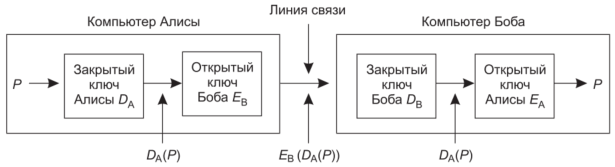
\includegraphics[width=0.8\textwidth]{signature.png}
    \attribution{Э. Таненбаум}
\end{center}

Тут Алиса хочет послать сообщение Бобу так, чтобы Боб мог убедиться, что сообщение действительно послала Алиса, и был бы уверен, что Алиса потом не будет отпираться, что послала сообщение. Алиса сначала шифрует сообщение своим закрытым ключом $D_A$, а затем, как обычно, шифрует то, что получилось, открытым ключом Боба $E_B$. Боб, получив такое сообщение, сначала применяет свой закрытый ключ, затем открытый ключ Алисы (он его знает, потому что Алиса заранее его опубликовала), получая тем самым исходное сообщение. Он точно знает, что автором была Алиса, потому что если бы автором был кто-то ещё, он бы не знал ключа $D_A$ и при применении $E_A$ получилась бы каша.

Ну а теперь, собственно, как не шифровать всё сообщение. Давайте сначала по нешифрованному сообщению посчитаем дайджест (Message Digest) --- хорошую хеш-функцию от сообщения, которая обладает таким свойством, что вычисляется по сообщению однозначно, но даже малое изменение сообщения (буквально в одном бите) до неузнаваемости меняет хеш-значение. При этом хеш-функция должна считаться быстро, и по данному хеш-значению должно быть невозможно получить исходное сообщение никак кроме как перебором (что с учётом того, что хеш-функция неизбежно теряет информацию, довольно безнадёжно, перебор даст лишь пару миллионов подходящих сообщений, которые даже похожи на правду). 

Дальше берём посчитанное хеш-значение и подписываем его описанным выше способом только его. Хеш-значение обычно небольшое (например, 20 байт), так что это можно сделать быстро. Адресату шлётся сообщение открытым текстом (например, библиотека .NET) и подписанный хеш (та самая цифровая подпись). Адресат по открытому сообщению сам считает хеш и применяет открытый клю автора к подписанному хешу, сличая то, что получилось. Если хеши одинаковые, то либо сообщение правда было отправлено кем надо и не менялось, либо злоумышленнику удалось подобрать такое сообщение, которое даёт точно то же хеш-значение, что и исходное, и при этом ещё и имеет смысл (что для достаточно хороших хеш-функций статистически маловероятно, настолько, что этим можно пренебречь).

Распространённые криптографические хеш-функции --- это MD5 (старая и уязвимая хеш-функция, коллизии подбираются атакой дней рождения за вполне конечное время), семейство функций SHA (SHA-1, SHA-2, SHA-3). SHA-1 тоже научились ломать, хоть это вычислительно гораздо сложнее, чем MD5, так что для практических цифровых подписей используются более криптостойкие SHA-2 и SHA-3 (SHA-3 относительно новая и не успела стать популярной). Все такие функции блочные, то есть подписываемое сообщение последовательно передаётся считалке хеша блоками (и обычно автоматически дополняется нулями до полной длины блока в конце). Конкретно SHA-1 применяет блоки по 512 бит и возвращает 160-битовый дайджест. Типичный подсчёт хеша --- это создать объект с алгоритмом криптографического хеша, в цикле пока сообщение не кончилось передавать ему блок за блоком, дальше вызвать метод <<верни хеш>>, который дополнит сообщение нулями, применит последний блок и вернёт посчитанный дайджест.

Применяются хеш-функции для цифровой подписи по такой схеме:

\begin{center}
    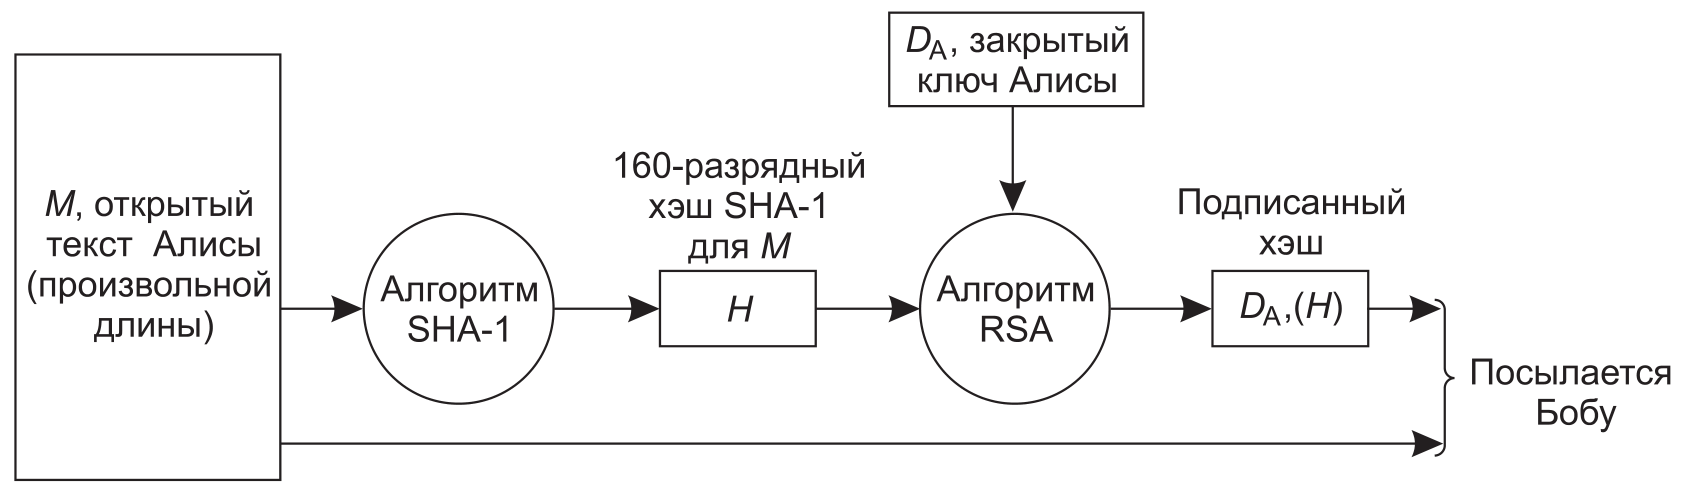
\includegraphics[width=0.85\textwidth]{sha1Signature.png}
    \attribution{Э. Таненбаум}
\end{center}

\subsection{Сертификаты}

Окей, теперь мы зная открытый ключ нашего собеседника без проблем проверим, что он тот, за кого он себя выдаёт, но как мы узнаем, что у нас на самом деле правильный открытый ключ нашего собеседника? Понятно, что мы могли бы получить его на флешке, но если бы для того, чтобы ходить во вконтактик, всем пришлось бы ехать за ключом в офис этой славной организации, никто бы вконтактиком не пользовался. Мы могли бы скачать открытый ключ со страницы нашего собеседника (например, того же vk.com), но злоумышленник довольно без проблем (до сих пор, несмотря на внедрение DNSSec!) может перехватить ваш запрос к странице и отправить вас на свою страницу, которая будет выглядеть точно так же, как vk.com, но содержать открытый ключ злоумышленника. А дальше --- атака Man In The Middle:

\begin{center}
    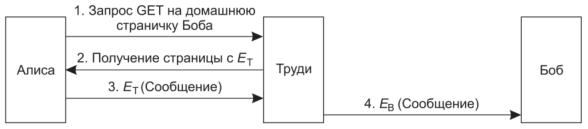
\includegraphics[width=0.8\textwidth]{manInTheMiddle.png}
    \attribution{Э. Таненбаум}
\end{center}

Чтобы такой беды не было, давайте, подписывать открытые ключи. Боб, публикуя свой открытый ключ, получает у кого-то, кому доверяет и Алиса, и Боб, сообщение, что это правда открытый ключ Боба, подписанное этим кем-то, кому все доверяют. Теперь Алиса, получив открытый ключ Боба, может проверить подпись в этом сообщении и убедиться, что это правда ключ Боба. Но что будет, если Труди (от английского inTruder) взломает страницу того, кому все доверяют, и подсунет свой ключ вместо его ключа, заставив тем самым Боба подписать своё ключ фальшивой подписью, которую Труди без проблем сможет подделать во время атаки Man In The Middle? Хм, давайте подпишем и этот ключ, и тот ключ, которым мы подписали этот ключ, и т.д. по цепочки, до Ключа, Которому Точно Все Доверяют. Такой ключ (точнее, несколько десятков их) могут быть вшиты в поставку операционной системы, браузера и т.п., так что при получении сообщения Алиса может проверить подписи по цепочке до ключа, который она получила от, например, Microsoft, и знает, что у злоумышленника вряд ли хватит денег, чтобы убедить Microsoft подсунуть фальшивый ключ.

Именно так работают \textit{сертификаты}. Сертификат --- это то самое сообщение, подтверждающее идентичность ключа (что-то вида <<предъявитель сего действительно является Иваном Ивановым, владельцем домена example.com>>), подписанное Certificate Authority (CA). Сертификаты имеют фиксированный формат, определяемый стандартом X.509, довольно ужасным, но по сути сводящемся к набору пар <<ключ-значение>>, хранящих информацию о владельце сертификата. Сертификаты бывают разные, от самых простых, что предъявитель сего владеет таким-то доменом, даже без указания имени хозяина, до сертификатов, выдаваемых интернет-магазинам сертификационными центрами, которые подтверждают, что владелец сертификата действительно может заниматься интернет-торговлей, не обманет и достаточно финансово устойчив, чтобы не обанкротиться, пока доставляет вашу покупку.  Понятно, что такие сертификаты стоят денег, и иногда немалых (и выдаются только на время, кстати).

CA верхнего уровня подписывают сертификаты CA уровнем ниже, чтобы те могли подписывать уже сертификаты конечных пользователей. Таким образом, получается цепочка сертификатов от конкретного пользователя до корневого CA, сертификаты которого общеизвестны и им все доверяют. При передаче сообщения передают всю цепочку сертификатов сразу, чтобы для проверки подписей вообще не требовалось выполнять сетевые запросы, благо сертификаты очень небольшие. Получатель может проследить, что все сертификаты в цепочке подписаны друг другом и цепочка заканчивается на сертификате, которому получатель точно доверяет, потому что, например, получил его десять лет назад вместе с новым компьютером. Такие доверенные сертификаты называются корневыми (root certificates) и хранятся в специальном хранилище в ОС любого компьютера.

Концептуально сертификат выглядит как-то так:

\begin{center}
    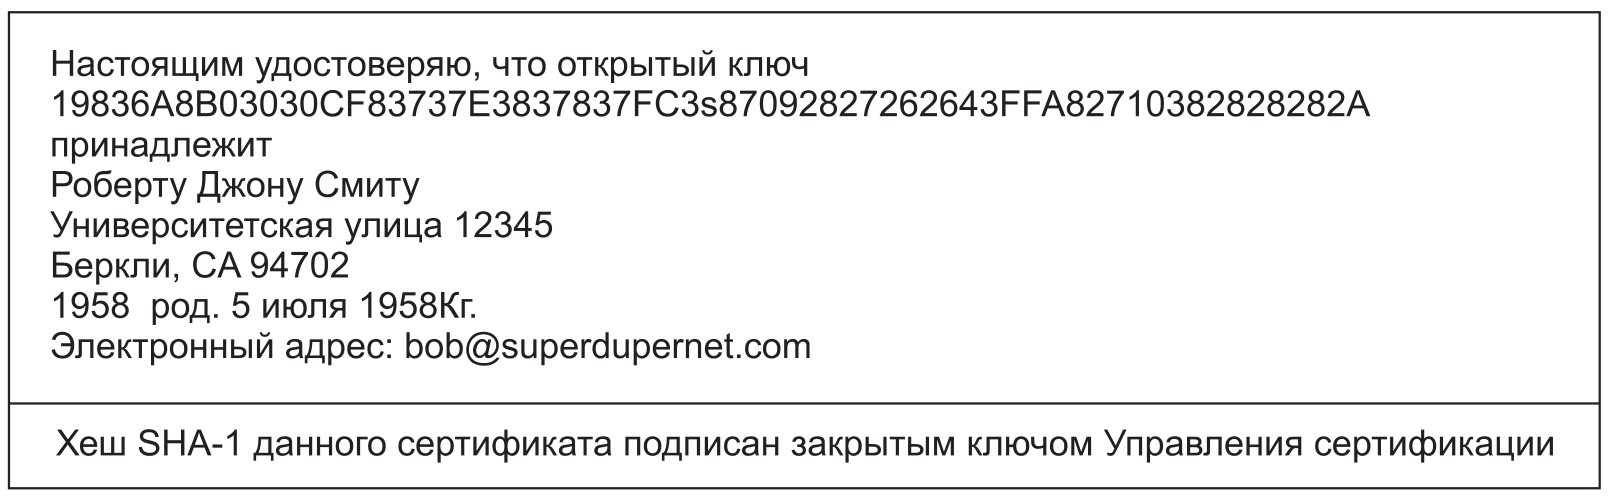
\includegraphics[width=0.65\textwidth]{certificate.png}
    \attribution{Э. Таненбаум}
\end{center}

То есть это подписанный файл, содержащий открытый ключ и некоторую информацию о его владельце (иногда удостоверяющий в каком-то смысле его личность, иногда просто декларирующий его права). На самом деле, файл с сертификатом содержит также и сертификат, подтверждающий ключ и права CА, и т.д., всю цепочку доверия до корневого сертификата:

\begin{center}
    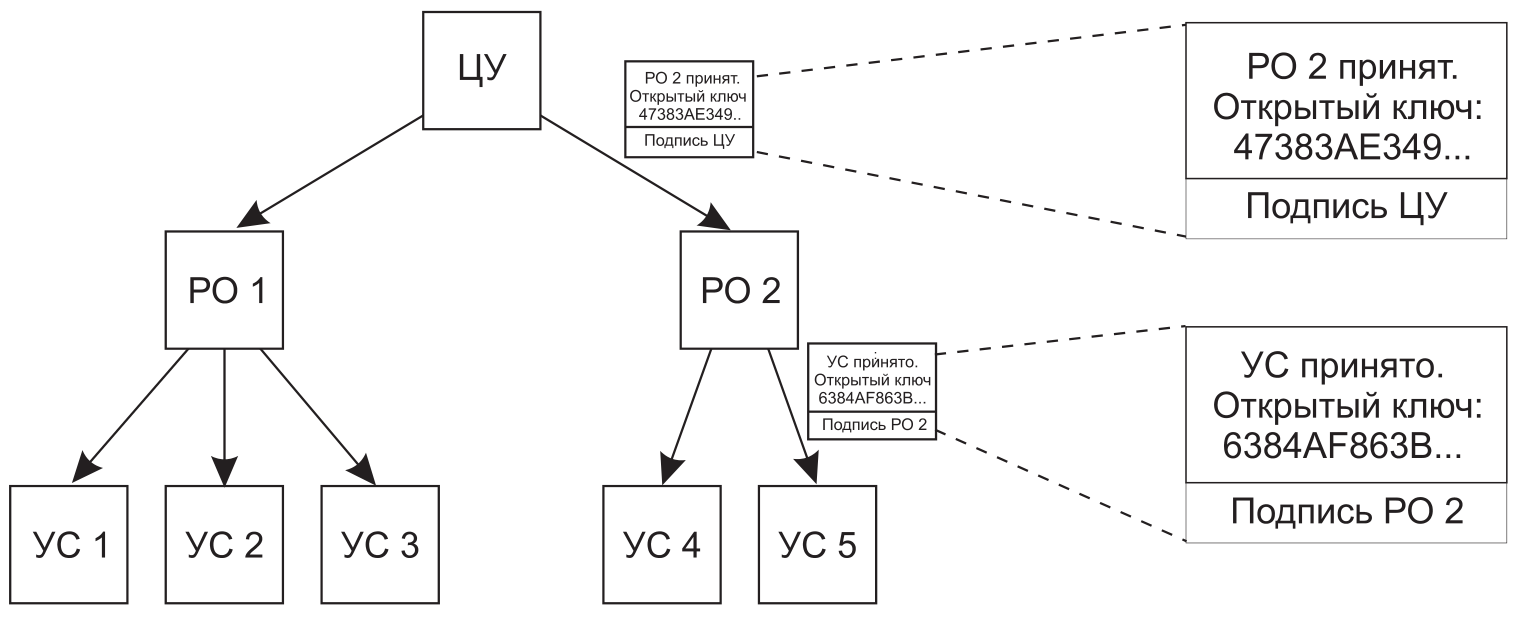
\includegraphics[width=0.85\textwidth]{certHierarchy.png}
    \attribution{Э. Таненбаум}
\end{center}

Хорошие сертификаты (которым все доверяют) стоят денег и требуют подтверждения, от показа паспорта до финансового аудита --- но если вы хотите заниматься электронной коммерцией, пользователи будут ожидать сертификата, в котром написано, что вы не склонны получить предоплату по заказу и убежать с ней на Канары. При этом сертификаты всегда выдаются на ограниченное время (обычно на год), при этом CA всегда может отозвать сертификат.

Поскольку настоящие сертификаты как минимум требуют что-то подтвердить, а как максимум стоят как недорогая иномарка, для отладки сетевых приложений используют \textit{самоподписанные} сертификаты. Это сертификат, который разработчик может сгенерировать сам, ему, понятное дело, никто не доверяет, потому что невозможно отследить его цепочку доверия до корневого сертификата, но разработчик может сам добавить такой сертификат в список доверенных. Тогда все приложения, пользующиеся системными сервисами проверки сертификатов, будут вынуждены ему доверять. Именно так работает Fiddler, когда дешифрует HTTPS-трафик, кстати. Visual Studio, кстати, умеет генерировать самоподписанные сертификаты: \url{https://docs.microsoft.com/en-us/windows/msix/package/create-certificate-package-signing}, но чаще это делают через инструменты библиотеки OpenSSL. 

А вот бесплатное CA, выдающее сертификаты, доказывающие владение доменом: \url{https://letsencrypt.org/}. Ему более-менее все современные браузеры доверяют, так что там можно получить вполне доверенный сертификат, которым можно защищать HTTPS-соединение. Код им подписывать не получится, но по крайней мере, шифровать соединение с сайтом вполне можно (а это необходимо для любого нормального протокола аутентификации). Так что в современном мире неиспользование HTTPS по причине дороговизны сертификата больше не является валидным.

Вот некоторые примеры мест, где сертификаты используются.

\begin{itemize}
    \item Протокол HTTPS, проверка идентичности сервера. Каждый раз при открытии соединения сервер обязан представить браузеру сертификат, доказывающий, что предъявитель сего действительно владеет доменным именем, на которое браузер зашёл. Браузер проверяет валидность сертификата, отслеживая цепочку доверия до корневых сертификатов, встроенных в сам браузер или в операционную систему. Это не спасёт от захода на какой-нибудь vК.com (где <<К>> русская), и это часто используют злоумышленники, но, по крайней мере, подсунуть DNS-системе фальшивый IPшник так уже не получится, и если пользователь будет внимательно смотреть, что у него в адресной строке, он не попадётся.
    \item Подписывание кода (Windows SmartScreen, Apple Code Signing). При запуске бинарника операционная система проверяет вшитый в него сертификат, и если не может отследить цепочку доверия, выдаёт предупреждение, что пользователь запускает что-то подозрительное. При этом сам код подписан ключом из сертификата, так что если какой-нибудь вирус в коде что-то поменял, цифровые подписи не сойдутся и система не станет запускать такую программу.
    \item Тот же принцип используется и в подписывании .NET-сборок (если кто не в курсе, .NET-программы состоят из .exe или .dll-файлов, даже под Linux, называемых сборками, и содержащими байт-код, который исполняется .NET-машиной при запуске). Подписанная ключом разработчика сборка называется сборкой \emph{с сильным именем} (потому что в таком случае fingerprint --- дайджест ключа --- используется как часть имени сборки для ресолва зависимостей при запуске программы). Опять-таки, цифровая подпись кода гарантирует, что 
    \begin{itemize}
        \item код не менялся с момента сборки,
        \item код собрал кто-то, кто заморочился получить сертификат, которым можно подписывать код
    \end{itemize}
    Такие сертификаты, впрочем, стоят денег, так что большая часть сборок в .NET не подписана (поскольку подписанные сборки могут использовать только подписанные сборки как зависимости, а почти все нормальные люди используют кучу бесплатных библиотек с открытым исходным кодом, которые никто за деньги подписывать не собирается).
\end{itemize}

Общая схема цифровой подписи кода в .NET такая (из отличной книжки J.Richter, CLR via C\#):

\begin{center}
    \includegraphics[width=0.6\textwidth]{dotNetCodeSigning.png}
    \attribution{J. Richter}
\end{center}

Публичный ключ разработчика вставляется в метаданные сборки, после этого по всей сборке кроме её заголовка считается криптографический хеш, подписывается приватным ключом разработчика и внедряется в метаданные сборки тоже. При запуске .NET-машина сама считает хеш всего, кроме заголовка, дешифрует его открытым ключом и сверяет с подписью в заголовке сборки. Если они не сошлись, программа не запускается (даже если это одна из сотни сборок, составляющих программу).

С технической точки зрения сертификаты хранятся в куче разных и несовместимых форматов. .pem, .p12, .pfx, .der, .cer, .crt. Причём разные системы и инструменты генерируют и принимают сертификаты в разных форматах. К счастью, их, как правило, довольно легко сконвертировать из одного в другой. Работать с сертификатами можно с помощью, например, PuttyGen под Windows (утилита, поставляющаяся вместе с очень популярной удалённой консолью Putty), или OpenSSL под любой операционной системой, есть также и специфичные для конкретных технологий средства (и .NET, JVM имеют свои утилиты для работы с сертификатами, JVM даже собственное хранилище).

Например, вот так можно сгенерировать самоподписанный сертификат с помощью OpenSSL:

\begin{minted}{bash}
openssl req -x509 -nodes -days 365 
    -newkey rsa:2048 -keyout privatekey.key 
    -out certificate.crt
\end{minted}

Тут мы говорим, что хотим сертификат в формате X509. Ключ -nodes говорит не шифровать сертификат симметричным шифром (угадайте каким) --- шифрование может применяться для дополнительной защиты приватного ключа. Если злоумышленник украдёт носитель с ключом, не зная ключа симметричного шифрования он не сможет быстро расшифровать сертификат. Однако за это придётся платить тем, что всякий раз, когда вам потребуется приватный ключ (например, чтобы что-нибудь подписать), придётся вводить ключ шифрования. -days 365 говорит, что сертификат имеет срок действия в год, -newkey rsa:2048 говорит, что мы хотим сгенерировать новый приватный ключ длиной в 2048 бит для алгоритма RSA. -keyout privatekey.key --- куда положить приватный ключ, -out certificate.crt --- куда положить сам сертификат с публичным ключом. Приватный ключ сохраняется у вас в Надёжном Месте\texttrademark и никуда никогда не отправляется, сертификат можно свободно распространять.

Например, добавить как доверенный в менеджере сертификатов под Windows:

\begin{center}
    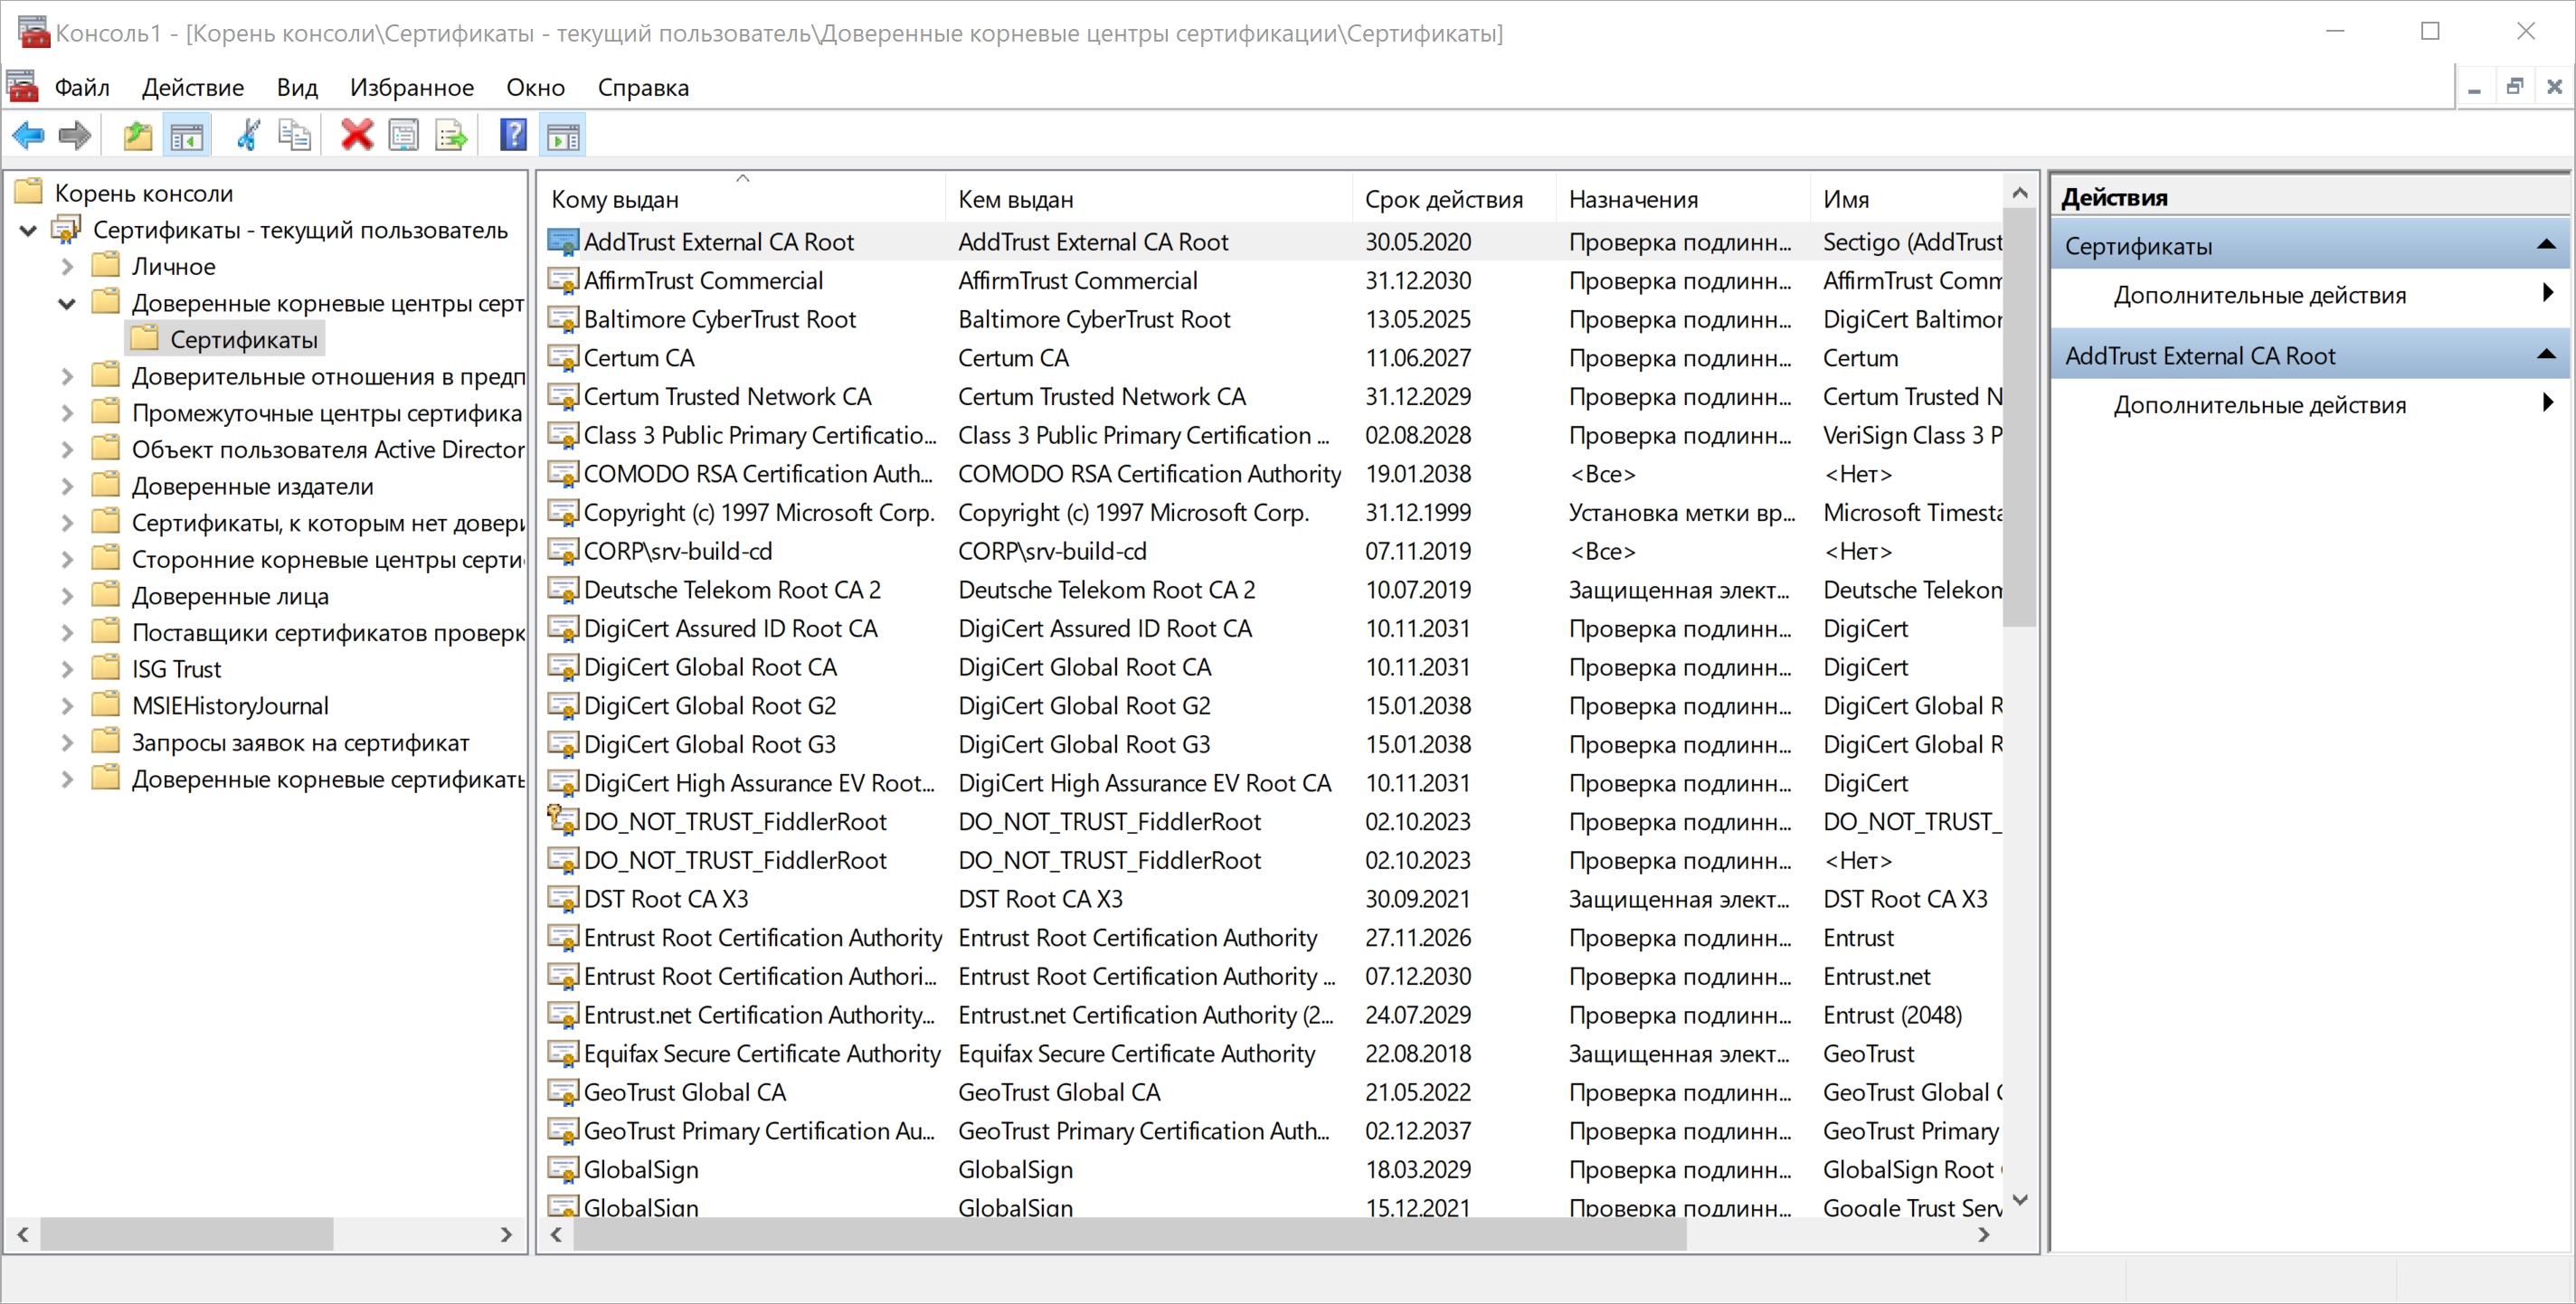
\includegraphics[width=0.95\textwidth]{windowsCertManager.png}
\end{center}

Чтобы тут оказаться, надо запустить Microsoft Management Console (Win-R, mmc), там File -> Add/Remove Snap-In, Certificates. Под Linux вроде достаточно кинуть сертификат в правильную папку и запустив утилиту, которая всё сделает (например, /usr/share/ca-certificates/ и update-ca-certificates). Там же (и в случае Windows в MMC, и под Linux в ca-certificates) можно посмотреть текущие установленные сертификаты во всех подробностях, и при необходимочти удалить лишние.

\section{Аутентификация}

Сертификаты позволяют нам убедиться, что публичный ключ принадлежит тому, кому должен, но следующая наша задача --- понять, говорим ли мы с тем, с кем хотим, или с кем-то ещё (даже если он может предъявить корректный сертификат). Кроме того, клиент может не иметь сертификата, и как-то должен доказать серверу, что он правда тот, за кого себя выдаёт. Оказывается, это довольно нетривиальная задача.

Самый простой случай аутентификации --- это когда оба собеседника имеют общий секретный ключ, который они могут предъявить друг другу (схема взаимного Challenge-Response). Однако поскольку в процессе нельзя этот ключ разгласить, а общение идёт по открытому каналу, это тоже не очень тривиально:

\begin{center}
    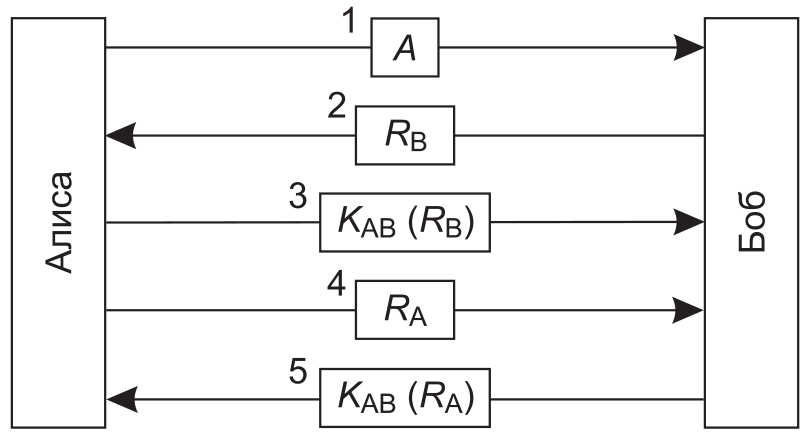
\includegraphics[width=0.5\textwidth]{challengeResponse.png}
    \attribution{Э. Таненбаум}
\end{center}

Алиса говорит Бобу, что она Алиса. Боб говорит <<докажи>>, посылая Алисе Challenge --- случайное число, которое Алиса должна зашифровать общим ключом (случайное число называется \emph{nonce}, number used once, оно должно для каждой операции быть сгенерено заново). Алиса отправляет зашифрованное число, Боб его расшифровывает и сверяет с тем, что он отправил, тем самым убеждаясь, что Алиса это Алиса. Дальше уже Алиса посылает челлендж Бобу, тоже nonce. Боб отвечает зашифрованным nonce, Алиса его расшифровывает и убеждается, что Боб это Боб.

Кажется, что этот протокол неоправданно сложный, и можно проще:

\begin{center}
    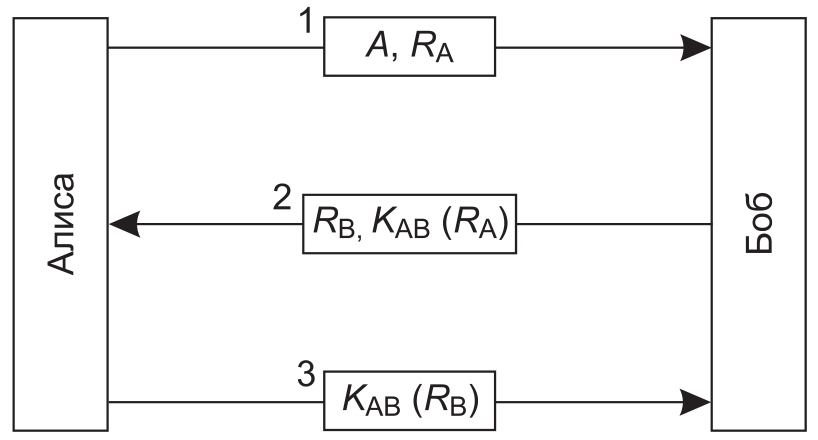
\includegraphics[width=0.5\textwidth]{simpleChallengeResponse.png}
    \attribution{Э. Таненбаум}
\end{center}

Алиса ведь может вместе со своей идентичностью сразу послать челлендж, Боб, отвечая на челлендж Алисы, может сразу ей послать свой челлендж, в остальном всё так же: три запроса вместо пяти, почти вдвое эффективнее. Однако внезапно оказывается, что такую схему можно взломать так называемой \emph{зеркальной атакой}: 

\begin{center}
    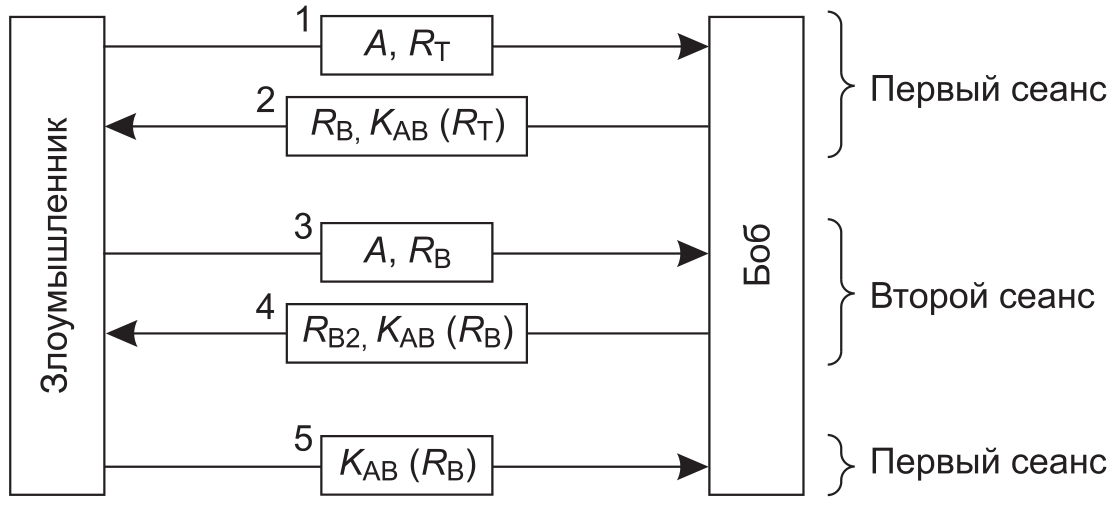
\includegraphics[width=0.65\textwidth]{mirrorAttack.png}
    \attribution{Э. Таненбаум}
\end{center}

Злоумышленник говорит, что он Алиса, и посылает Бобу челлендж. Боб, ни о чём не догадываясь, отвечает и посылает свой челлендж в ответ. Злоумышленник открывает \emph{вторую} сессию с Бобом, говорит, что он Алиса (не обязательно Алиса, чтобы Боб ничего не заподозрил, просто кто-то) и посылает в качестве челленджа nonce Боба. Боб, ничего не подозревая, шифрует nonce, отправляет его <<Алисе>>, а <<та>> отвечает им же на первый челлендж Боба и закрывает второе соединение. Всё, злоумышленник доказал Бобу, что он Алиса.

Зеркальной атаки легко избежать разными способами, от запрета параллельных соединений (что проблематично в случае реальных веб-серверов) до выбора nonce-ов из разных диапазонов. Но суть в том, что внешне выглядящий правильным протокол аутентификации оказывается полностью уязвим для довольно неочевидной атаки, о которой ни один нормальный человек так сходу и не подумал бы. В общем, разработать корректный протокол аутентификации сложнее, чем это может показаться.

Конкретно в этом случае правильный протокол всё-таки можно сделать из всего трёх сообщений, вот так:

\begin{center}
    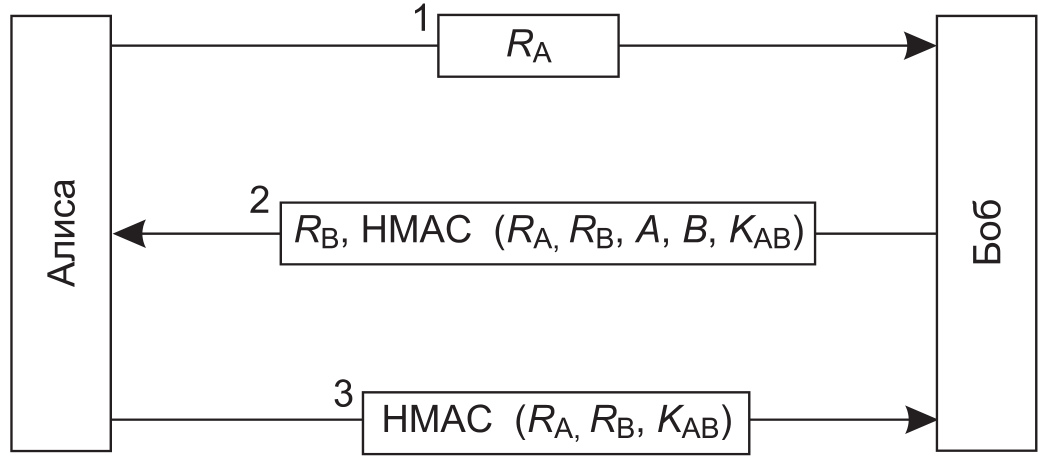
\includegraphics[width=0.6\textwidth]{hmacs.png}
    \attribution{Э. Таненбаум}
\end{center}

Тут используется Hashed Message Authentication Code (HMAC), тоже довольно важная для криптографии штука. Это криптографический хеш, считающийся от переданных ему параметров (например, просто конкатенации их битовых последовательностей). Теперь Боб не раскрывает Алисе существенную информацию до того, как она доказала, что она Алиса, но оба участника взаимодействия всё ещё могут проверить идентичность друг друга: Боб отвечает на запрос Алисы об аутентификации своим челленджем и HMAC-ом, посчитанным от nonce-а Алисы, nonce-а Боба, идентичностей Алисы и Боба и их общего секретного ключа. Алиса из всего этого не знает только nonce Боба, но он передаётся вместе с HMAC, так что Алиса без проблем может посчитать свой хеш и проверить, что он совпадает с хешем Боба. Поскольку только Боб знает общий секретный ключ, злоумышленник не сможет быстро подобрать такой хеш, чтобы он совпал с ожидаемым, так что если хеш совпал, то Алиса знает, что Боб --- это Боб. Алиса отвечает Бобу своим HMACом, посчитанным от nonce-ов Алисы и Боба, и секретного ключа --- вся эта информация есть у Боба, а злоумышленнику не хватает секретного ключа, так что Боб может сверить хеши и понять, что Алиса --- это Алиса.

\subsection{Basic Authentication}

В реальной жизни, однако, для прикладного программиста всё несколько проще. Секретность передачи обеспечивается транспортным уровнем --- если подключение к серверу выполняется по протоколу HTTPS, прочитать трафик злоумышленнику и так не удастся, причём сервер уже доказал (в каком-то смысле), что он тот, за кого себя выдаёт. Поэтому клиент просто открытым текстом посылает свои логин и пароль серверу, они шифруются самим HTTPS и безопасно доставляются серверу.

В такой схеме есть два подводных камня --- что будет, если взломают клиент, и что будет, если взломают сервер.

\begin{itemize}
    \item Чтобы не держать в памяти логин/пароль пользователя, их принято затирать нулями сразу после передачи первого сообщения. Сервер отвечает токеном доступа (Access Token) --- некоей случайно сгенерированной строкой, которую запоминают и сервер, и клиент (либо сервер не запоминает, а просто имеет возможность проверить, что это и правда он недавно сгенерил). Дальше клиент предъявляет в последующих запросах не логин и пароль, а только Access Token. Даже если клиент окажется взломан и Access Token украдут, он имеет ограниченное время жизни, и можно надеяться, что пока его крадут, успеет <<протухнуть>>. Законный владелец живого Access Token-а может его продлить, чтобы не авторизоваться снова по истечении времени жизни токена. В ответ на запрос о продлении ему выдадут новый (так что злоумышленнику придётся начинать всё с начала).
    \item Сервер должен как-то понимать, что предъявленные ему логин и пароль принадлежат законному пользователю. Наивное решение --- хранить пары <<логин-пароль>> на сервере (например, в базе данных), в надежде, что сервер-то не взломают. Однако так делать, естественно, нельзя --- базу украдут, и, поскольку пользователи часто используют один и тот же пароль для доступа к разным сервисам, это позволит злоумышленнику получить доступ к целой куче информации пользователей. Поэтому в базе хранятся не сами пароли, а их криптографические хеши --- сервер может посчитать хеш от пароля при аутентификации и убедиться, что он совпадает с хешем в базе, а злоумышленник, украв базу, получает только хеши. По которым как бы не может восстановить пароль. Однако злоумышленнику на помощь приходят <<радужные таблицы>> --- гигантские таблицы с предпосчитанными хешами для часто используемых паролей. Теперь можно пробежаться по базе, найти знакомые хеши и понять, какие пароли были у их пользователей. Чтобы <<радужные таблицы>> оказались бесполезны, на стороне сервера используется <<соль>> (salt) --- это просто случайное число, которое дописывается к паролю перед тем, как посчитать его хеш. Соль тоже хранится в базе, вместе с хешем пароля, прямо открытым текстом, так что при аутентификации можно <<посолить>> присланный законным пользователем пароль и сверить хеши. Злоумышленник же теперь, зная хеш и соль, не может восстановить пароль даже радужными таблицами (разве что у него есть 4 миллиарда разных таблиц, по одной для каждого возможного значения соли, но это совсем-совсем непрактично).
\end{itemize}

\subsection{Аутентификация с открытым ключом}

Если у нас есть сертификаты, то можно вообще никакие секреты не хранить, а использовать схему аутентификации с открытым ключом (правда, нам потребуется третья сторона, которой все доверяют, и которая будет сертификаты хранить). Работает аутентификация с открытым ключом так:

\begin{center}
    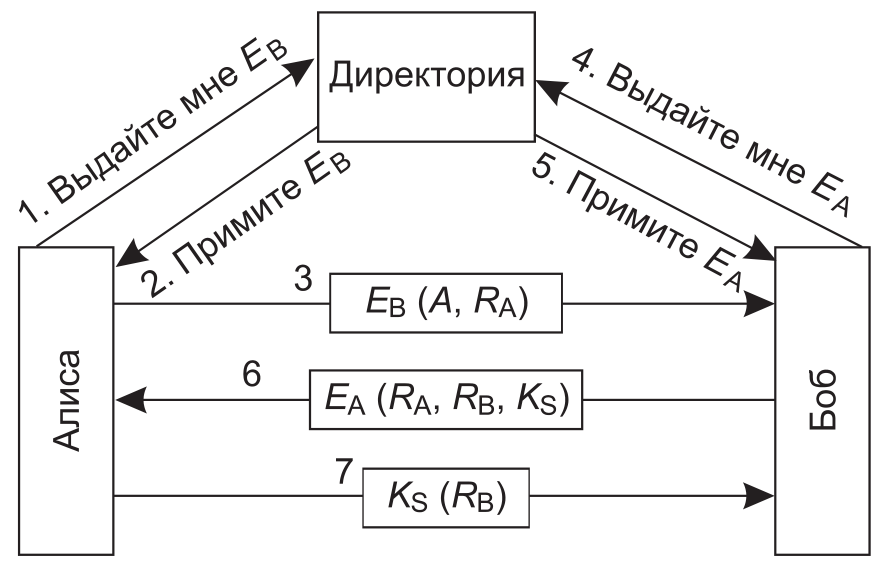
\includegraphics[width=0.6\textwidth]{openKeyAuthentication.png}
    \attribution{Э. Таненбаум}
\end{center}

Здесь $E_A$ и $E_B$ --- открытые ключи Алисы и Боба, которые и Алиса, и Боб откуда-то знают, например, запрашивают при установлении соединения из какого-то доверенного хранилища. Дальше Алиса выбирает nonce $R_A$ и шифрует его открытым ключом Боба, вместе со своей идентичностью. Боб отвечает $R_B$ --- nonce Боба, расшифрованным $R_A$ и выбранным Бобом симметричным ключом $K_S$, всё это шифруется открытым ключом Алисы. Алиса проверяет, что Боб --- это Боб, потому что не Боб не смог бы прочитать $R_A$, и отвечает $R_B$, зашифрованным симметричным ключом $K_S$. Боб в этот момент понимает, что Алиса --- это Алиса, потому что никто больше не смог бы прочитать $K_S$ и $R_B$.

В реальной жизни такая схема используется довольно редко, потому что требует наличия ключа у обоих участников взаимодействия, что порождает проблемы хранения приватной части ключа и использования его на разных устройствах. И это не спасает от атаки посредника (как в случае Диффи-Хеллмана, злоумышленник может подсунуть Алисе и Бобу свой ключ вместо ключа собеседника), поэтому и нужна доверенная директория. В реальной жизни сервер аутентифицируется обычным сертификатом средствами HTTPS, а открытый ключ клиента каким-то безопасным образом (например, на флешке, чтобы его не подменили по пути) доставляется на сервер и хранится там (то есть серверу ниоткуда ключ получать не надо). Даже если сервер взломают, злоумышленник получит открытые ключи всех пользователей, которые, в общем-то, и так не секрет. Обратите внимание, что клиенту не нужен полноценный сертификат, если сервер доверяет открытому ключу.

Так, например, работает SSH-аутентификация на GitHub, Yandex.Cloud и многих серверах, администрируемых по SSH.

\section{Авторизация}

\subsection{OAuth 2}

Второе, с чем надо разобраться --- это с авторизацией. Хорошо, Алиса и Боб смогли подтвердить идентичность друг друга, но Алиса хочет зайти на файловое хранилище и скачать оттуда файл, а Боб должен проверить, что она имеет на это право. Боб мог бы сам владеть и файловым хранилищем, и держать у себя таблицу, в которой написано, что Алиса имеет право делать, а что нет, и это бы даже хорошо работало, если бы Алиса только для этого и пользовалась интернетом. Но подумаем об обычном пользователе, который зареган на тысяче ресурсов. Если к каждому надо придумывать свой логин и пароль, можно сойти с ума. Если каждый ресурс знает логин и пароль пользователя, то если взломают хоть один, взломают и все остальные.

Поэтому появился протокол OAuth (тут речь пойдёт про OAuth 2, используемый ныне). Этот протокол позволяет разрешить пользование ресурсом, не раскрывая хозяину ресурса логин и пароль пользователя. Например, можно войти на сторонний ресурс по аккаунту в Google или аккаунту в VK, не сообщая при этом ресурсу никакой ценной информации о себе, не говоря уж о логине и пароле. Так можно помнить только пароль от Google и ходить на все остальные сайты, умеющие в OAuth, по нему. Светлая цель разработки такого протокола была вообще в том, чтобы был некий глобальный сервис аутентификации, которому все доверяют, и который бы позволял проверить идентичность пользователя и дать доступ ко всем остальным сайтам интернетов, но, во-первых, с <<которому все доверяют>> возникли проблемы, во-вторых, когда это человечество о чём-то хорошем договорилось.

Работает протокол примерно как на картинке из стандарта (RFC 6749):

\begin{center}
    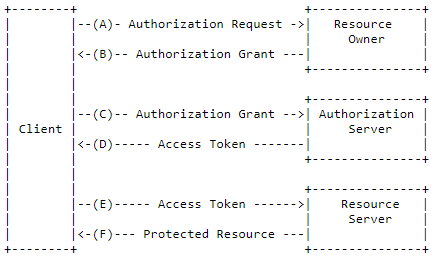
\includegraphics[width=0.6\textwidth]{oauth.png}
    \attribution{RFC 6749}
\end{center}

Client --- это приложение, которое хочет работать с каким-то ресурсом (например, браузерный клиент гуглодиска). Resource Owner --- это пользователь (человек), который может разрешить или не разрешить клиенту доступ к ресурсу. Authorization Server --- это то место, где разрешение на доступ к ресурсу можно обменять на Access Token, если Resource Owner реально имеет право на доступ к ресурсу. Дальше мы можем с этим Access Token-ом пойти на ресурсный сервер и предъявить уже Access Token, чтобы пользоваться ресурсом, не авторизуясь на нём ещё раз. Аутентификация и авторизация проводится только один раз, на Authorization Server-е, выдаваемый им токен устроен так, что Resource Server может легко проверить его валидность и то, что клиент действительно имеет право выполнять запрашиваемую операцию (очередное применение криптографических хешей, кстати).

Чаще всего протокол OAuth 2 используется в режиме Authorization Code, когда клиент не запрашивает у владельца ресурса авторизацию напрямую, а перенаправляет его на Authorization Server, где владелец аутентифицируется и авторизуется. При этом логин/пароль пользователя видит только Authorization Server, даже клиент не имеет к ним доступа. Authorization Server затем отвечает клиенту, отправляя ему Access Token (для чего используется некая магия с URL-ами). С Access Token также связан некий Scope --- набор прав, которые этот Access Token предоставляет предъявителю (например, только чтение или чтение и запись). При этом Access Token имеет свойство протухать через некоторое небольшое время (чтобы если злоумышленник перехватит Access Token, он с меньшей вероятностью мог воспользоваться ресурсом), поэтому клиенту также обычно выдаётся Refresh Token --- токен, который можно обменять на новый Access Token, когда старый протухнет. Refresh Token живёт подольше (обычно от нескольких дней до пары месяцев) и его можно продлять, так что если пользователь часто пользуется ресурсом (например, ходит во вконтакт каждый день), ему вообще не надо авторизовываться. Refresh Token передаётся по сети довольно редко, так что несмотря на то, что он важнее, вероятность, что его перехватят, меньше. Напомним, что всё происходит по HTTPS, так что чтобы получить хоть один токен, сначала надо взломать относительно неломаемый протокол. А если его всё-таки взломают, Refresh Token часто можно вручную отозвать.

Пример OAuth2 в реальной жизни --- это Google OAuth 2.0, работающий как Authorization Server для всех сервисов Google и для кучи сторонних приложений. Чтобы им воспользоваться, вам надо сначала пойти в Google Developer Console и зарегистрировать своё приложение, которое хочет пользоваться Google OAuth. Там вам дадут Client ID и Client Secret, которые приложение должно предъявлять серверу авторизации каждый раз, это идентифицирует приложение, делающее запрос (для десктопных и мобильных приложений Client Secret на самом деле не секрет, его может узнать любой законный пользователь приложения, подсмотрев трафик. Для веб-приложений Client Secret может храниться на сервере, и там его достать гораздо сложнее). Дальше, в коде приложения, вы предъявляете Client ID и Client Secret при авторизации в Google OAuth, и запрашиваете код акторизации, передавая ресурс и Scope, к которым хотите получить доступ (например, к гуглодиску на чтение). В этот момент пользователя перенаправляют на страницу логина в аккаунт Google, где он логинится как обычно, уже без помощи вашего клиента (и по идее ваш клиент ничего не знает про эту часть процедуры, так что логина и пароля пользователя не видит). При необходимости пользователю показывают Consent Screen, где говорят, что приложение такое-то хочет от такого-то ресурса такие-то права. Consent Screen конфигурируем в Google Developer Console, однако если ваше приложение не прошло ревью в Google, пользователя предупредят, что это что-то левое и потенциально небезопасное.

При успешном логине вашему приложению отвечают кодом авторизации (каким-то образом, например, делая редирект на заданный URL, или отправляя на специально поднятый для этого мини-сервер на компьютере клиента). Дальше код аторизации можно обменять на токен авторизации и refresh token. Первый надо предъявлять при каждом запросе к ресурсу, второй --- чтобы получить новый токен авторизации, если старый истёк. На диаграмме последовательностей UML это выглядит как-то так:

\begin{center}
    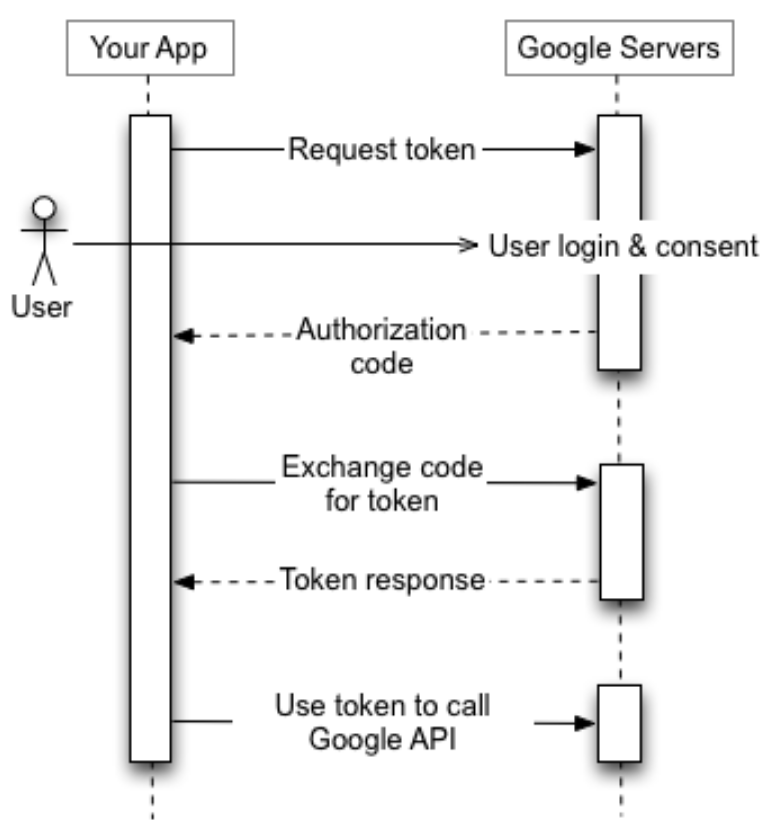
\includegraphics[width=0.4\textwidth]{googleOAuth.png}
    \attribution{\url{https://developers.google.com}}
\end{center}

\section{HTTPS}

Собственно, сертификаты используются очень много где, но в контексте сетевых приложений они наиболее важны для установки HTTPS-соединения. HTTPS --- это обычный протокол HTTP, использующий Secure Sockets Layer, или SSL, в качестве протокола уровня представления. Установление соединения по HTTPS включает в себя аутентификацию сервера на клиенте как раз через цепочку сертификатов. Клиент не должен доказывать свою идентичность серверу (об этом потом позаботится аутентификация, уже когда соединение будет установлено), но если сервер не сможет убедить клиента, что он правда тот, на который клиент пытается зайти (в смысле доменного имени), соединение даже установлено не будет.

Вот так примерно устроено установление соединения по HTTPS:

\begin{center}
    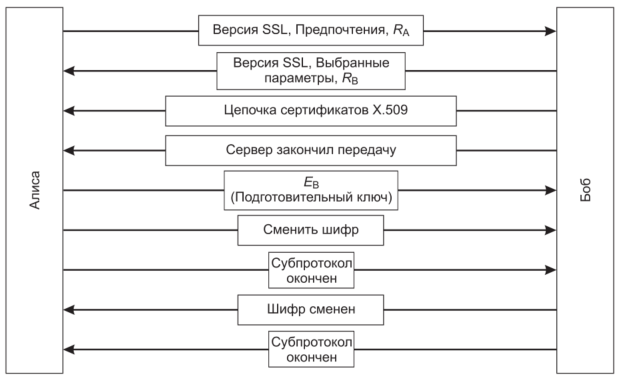
\includegraphics[width=0.8\textwidth]{ssl.png}
    \attribution{Э. Таненбаум}
\end{center}

Сначала Алиса и Боб договариваются о версии SSL и обмениваются одноразовыми ключами (nonce-ами, для предотвращения атаки повтором), затем Боб отправляет свою цепочку сертификатов, чтобы доказать, что он правда Боб, затем Алиса шифрует открытым ключом Боба подготовительный ключ для симметричного шифрования (который тоже выбирает случайно, используя nonce-ы), Боб, зная свой закрытый ключ и оба nonce-а, расшифровывает симметричный ключ, подтверждает получение Алисе и переходит на симметричный шифр с этим ключом. Ненадолго, впрочем, HTTPS предполагает частую смену симметричного ключа во избежание статистических атак.

Далее работает транспортный субпротокол с симметричным шифром: 

\begin{center}
    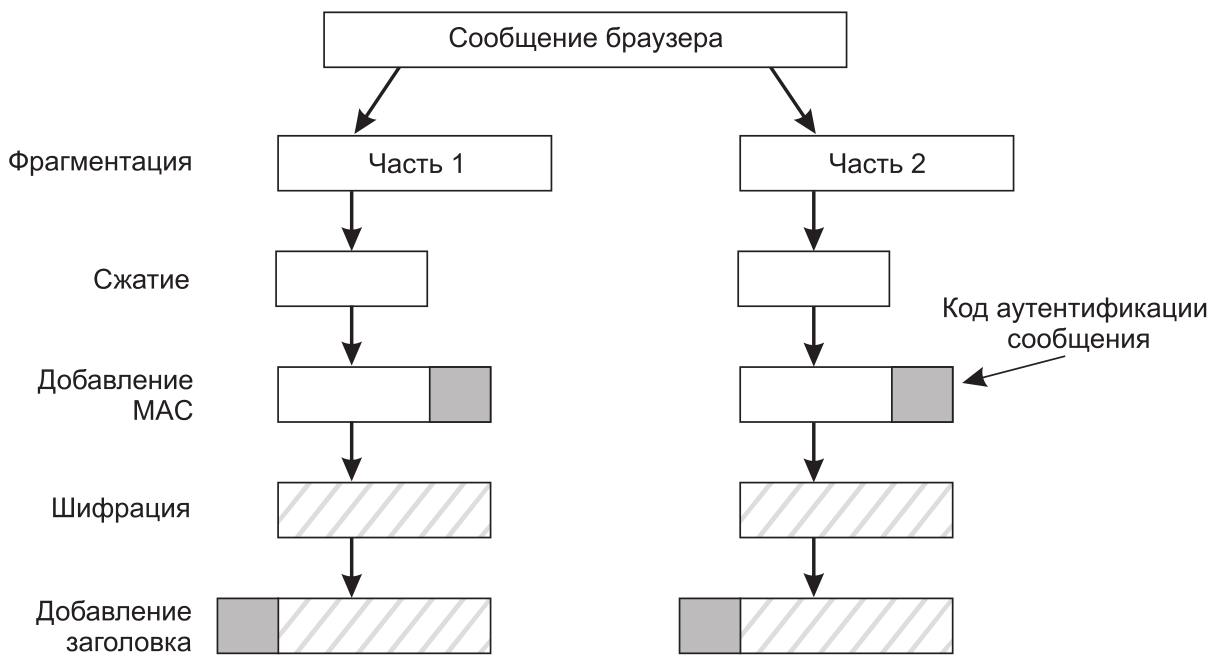
\includegraphics[width=0.6\textwidth]{sslCommunication.png}
    \attribution{Э. Таненбаум}
\end{center}

Сообщение разбивается на фрагменты, жмётся (обычным gzip-ом, обычно, для экономии трафика), к результату добавляется Hashed Message Authentication Code (HMAC) --- просто хеш сжатого сообщения, чтобы его нельзя было поменять. Дальше результат шифруется, добавляются заголовки и уже отправляются по TCP. Для шифрования используется обычно либо Triple DES в режиме Cipher Block Chaining, либо RC4\footnote{Rivest Cipher 4, несмотря на похожесть названия на RCA, это симметричный шифр.}, для хеширования сообщений SHA-1 или MD5. Как видим, не то чтобы супернадёжно, но в реальном времени, и поскольку симметричный ключ меняется автоматически и довольно часто, взломать такой протокол довольно тяжело.

Однако же сейчас SSL в чего чистом виде практически не встретить, как раз по соображениям криптостойкости. На смену ему пришёл протокол TLS (Transport Layer Security) различных версий (у них на самом деле сложная история, TLS начинался как копия SSL, намеренно сделанная несовместимой). В TLS используются более суровые шифры (AES в основном), и более интересные хеш-функции (включая, судя по Википедии, хеш ГОСТ Р 34.11-94), оставаясь при этом в рамках, разрешённых большинством государств для гражданской криптографии. Для всех практических применение, тем не менее, при аккуратном использовании TLS можно считать достаточно надёжным.

\section{Атака <<DNS Spoofing>>}

В этой лекции не раз делались оговорки, что Алиса должна знать, что Боб это Боб, что есть атака посредника, что могут подсунуть не тот сертификат или не тот ключ, и т.д. Но если вы сами ввели в адресной строке браузера vk.com и нигде не опечатались, вы же должны оказаться на ВКонтакте и ничто не может пойти не так, да? Нет. Злоумышленник может направить ваш браузер на свою копию ВКонтакта, где вы авторизуетесь и потеряете тем самым свой аккаунт на настоящем ВКонтакте. При этом даже не трогая никак ни ваш браузер, ни вообще ваш компьютер. 

Чтобы понять, как такое возможно, надо вспомнить, что браузер, перед выполнением собственно запроса, делает преобразование из доменного имени в IP-адрес, с помощью службы DNS. И что DNS устроены иерархически, чтобы не перегружать запросами корневые сервера, так что, как правило, у каждого провайдера есть свой собственный DNS-сервер, помнящий часто используемые адреса. Он-то и может стать объектом атаки, и его можно обмануть, даже не получая над ним никакого контроля. Как это делается (это и называется <<DNS Spoofing>>):

\begin{center}
    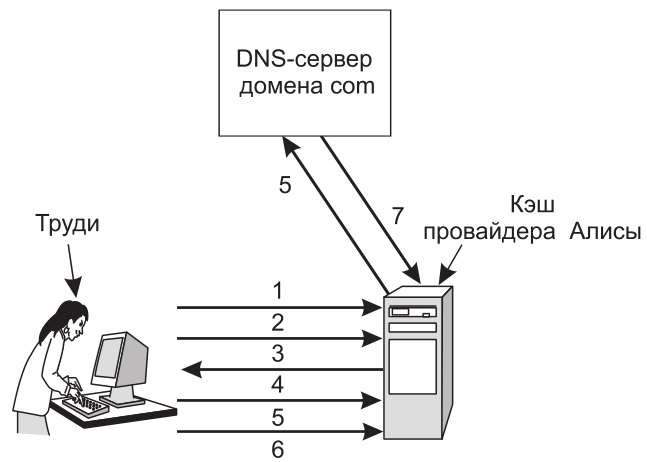
\includegraphics[width=0.45\textwidth]{dnsSpoofing.png}
    \attribution{Э. Таненбаум}
\end{center}

Допустим, Алиса хочет попасть на bob.com. Злоумышленница Труди, зная о намерении Алисы, регистрирует доменное имя trudy-the-intruder.com, поднимает там свой DNS-сервер и проводит некоторые подготовительные мероприятия: 

\begin{enumerate}
    \item Сначала она делает запрос на foobar.trudy-the-intruder.com через DNS-сервер провайдера Алисы (чтобы trudy-the-intruder.com попал в кеш провайдера, при этом существование foobar опционально, важно, чтобы DNS-сервер провайдера озаботился существованием домена trudy-the-intruder.com).
    \item Дальше она делает запрос www.trudy-the-intruder.com (чтобы получить следующий порядковый номер провайдера).
    \item DNS-сервер провайдера Алисы делает запрос к DNS, обслуживающему домен trudy-the-intruder.com, чтобы узнать адрес машины www. К DNS Труди.
    \item DNS Труди не торопится отвечать, вместо этого Труди делает запрос к bob.com через DNS провайдера.
    \item DNS провайдера, не зная, кто такой bob.com (ну, мы надеемся), делает запрос к DNS зоны com.
    \item И вот в этот момент DNS Труди отвечает DNS провайдера Алисы, но не про www.trudy-the-intruder.com, а про bob.com, подделав также и номер запроса из шага 5 (мы его узнали на шаге 3). Вместо реального IP bob.com Труди указывает свой IP.
    \item DNS зоны com отвечает DNS провайдера, сообщая настоящий адрес bob.com, но уже поздно, потому что провайдер думает, что уже получил ответ, и это просто дубликат ответа.
\end{enumerate}

Теперь, может, через пару дней, Алиса выходит в интернет и спокойно идёт на bob.com, попадая при этом на машину Труди. Где крутится сайт, неотличимый внешне от bob.com (потому что Труди ничего не стоит получить оттуда все HTML-ки, картинки, стили и даже скрипты), однако ворует пароли или отдаёт Алисе поддельный публичный ключ:

\begin{center}
    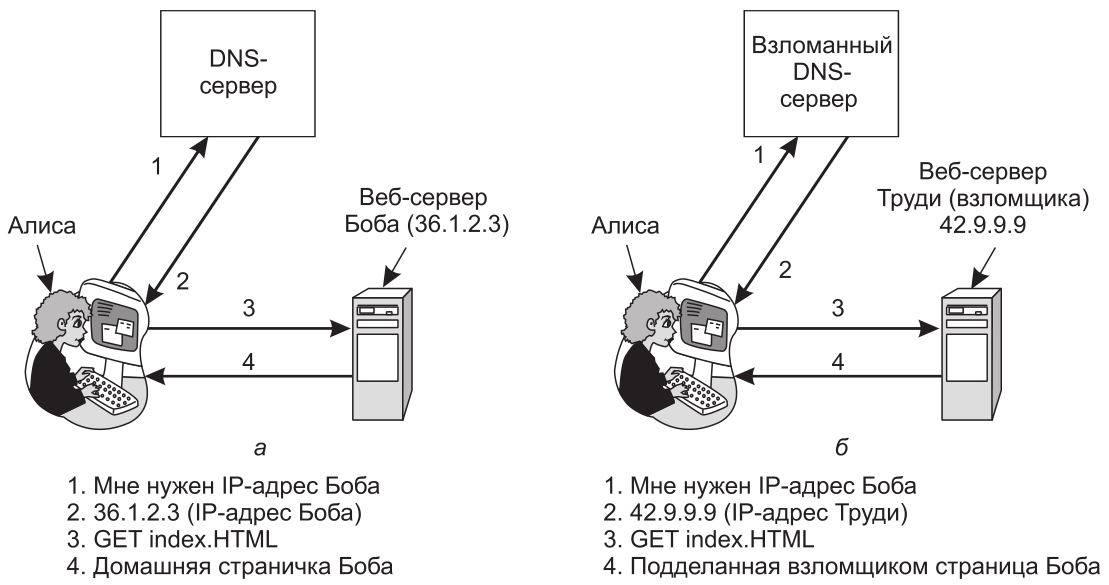
\includegraphics[width=0.9\textwidth]{dnsSpoofingResult.png}
    \attribution{Э. Таненбаум}
\end{center}

К счастью, нынче активно внедряется протокол DNSSEC, который использует очень простую идею --- а давайте подписывать ответ DNS-сервера сертификатом сервера. Так что Труди не получится подделать ответ от DNS-сервера зоны com, потому что она не может подписать свой ответ его ключом. Но проблема DNSSEC в том, что DNS-запросов в сети делается огромное количество, так что при полном переходе интернета на DNSSEC производительность сетей заметно просядет. Поэтому корневые DNS-сервера DNSSEC давно используют, остальные --- как повезёт.

\section{Инструменты сетевой отладки}

Наконец, немного про инструменты отладки сетевых приложений, которые могут показать, кто кому какие пакеты шлёт, какие средства безопасности использует, и, в большинстве случаев, прочитать даже зашифрованный трафик, уходящий/приходящий на вашу машину. 

\begin{itemize}
    \item Первый и самый полезный инструмент --- это сам браузер. При пользовании веб-приложением можно нажать F12 (или что-то такое, в зависимости от браузера, но любой браузер так умеет) и посмотреть, что кто куда передаёт и что ему отвечают. Однако если вы интересуетесь не браузерным приложением, так не получится.
    \item На помощь придёт Fiddler --- это кроссплатформенный отладчик HTTP/HTTPS-трафика, который устанавливается как системное прокси и просит все приложения слать трафик через себя (на самом деле это делает сама операционная система, конечно). Правда, есть приложения, которые работать с прокси не умеют или не хотят, их трафик Fiddler не увидит. Ещё Fiddler умеет дешифровывать HTTPS-трафик, делая самую настоящую атаку посредника. Он при первом включении HTTPS-отладки предложит добавить в доверенные сертификаты операционной системы свой сертификат и все HTTPS-соединения будет подписывать этим сертификатом, потом сам отправляя запрос уже правильному адресату и используя правильный сертификат (адресата). Поскольку сертификат Fiddler доверенный, у приложений, работающих на вашем компьютере, нет оснований ему не доверять, и они спокойно шлют свои пакеты по такому соединению. Ещё Fiddler умеет показывать пакеты в разных форматах (JSON, XML, прямо рендерить HTML, как браузер), умеет модифицировать пакеты, повторять отправку и т.д. и т.п. На самом деле, Fiddler --- стандарт де-факто в отладке распределённых приложений, так что must have.
    \item Однако Fiddler умеет только HTTP/HTTPS, а если вам надо ловить сырые TCP или UDP-пакеты, или вдруг посмотреть, что именно шлёт приложение вашему любимому iPhone по USB, Fiddler никак не поможет. Тогда можно воспользоваться Wireshark --- он уже не прокси, а набор драйверов, ставящихся в ядро операционной системы поверх стандартных (в Windows, например, есть понятие драйвера-фильтра, который <<надевается>> поверх другого драйвера), и красивого GUI для отображения результатов. Wireshark может читать в принципе всё, что кто-то куда-то пытается отправить, но несколько сложнее в использовании, поэтому используется, когда Fiddler не справляется, а не вместо него.  Wireshark уже скорее не must have, а must know.
\end{itemize}

\end{document}
